% Options for packages loaded elsewhere
\PassOptionsToPackage{unicode}{hyperref}
\PassOptionsToPackage{hyphens}{url}
%
\documentclass[
]{book}
\usepackage{amsmath,amssymb}
\usepackage{lmodern}
\usepackage{iftex}
\ifPDFTeX
  \usepackage[T1]{fontenc}
  \usepackage[utf8]{inputenc}
  \usepackage{textcomp} % provide euro and other symbols
\else % if luatex or xetex
  \usepackage{unicode-math}
  \defaultfontfeatures{Scale=MatchLowercase}
  \defaultfontfeatures[\rmfamily]{Ligatures=TeX,Scale=1}
\fi
% Use upquote if available, for straight quotes in verbatim environments
\IfFileExists{upquote.sty}{\usepackage{upquote}}{}
\IfFileExists{microtype.sty}{% use microtype if available
  \usepackage[]{microtype}
  \UseMicrotypeSet[protrusion]{basicmath} % disable protrusion for tt fonts
}{}
\makeatletter
\@ifundefined{KOMAClassName}{% if non-KOMA class
  \IfFileExists{parskip.sty}{%
    \usepackage{parskip}
  }{% else
    \setlength{\parindent}{0pt}
    \setlength{\parskip}{6pt plus 2pt minus 1pt}}
}{% if KOMA class
  \KOMAoptions{parskip=half}}
\makeatother
\usepackage{xcolor}
\IfFileExists{xurl.sty}{\usepackage{xurl}}{} % add URL line breaks if available
\IfFileExists{bookmark.sty}{\usepackage{bookmark}}{\usepackage{hyperref}}
\hypersetup{
  pdftitle={Interactive maps with leaflet},
  pdfauthor={Rex Parsons},
  hidelinks,
  pdfcreator={LaTeX via pandoc}}
\urlstyle{same} % disable monospaced font for URLs
\usepackage{color}
\usepackage{fancyvrb}
\newcommand{\VerbBar}{|}
\newcommand{\VERB}{\Verb[commandchars=\\\{\}]}
\DefineVerbatimEnvironment{Highlighting}{Verbatim}{commandchars=\\\{\}}
% Add ',fontsize=\small' for more characters per line
\usepackage{framed}
\definecolor{shadecolor}{RGB}{248,248,248}
\newenvironment{Shaded}{\begin{snugshade}}{\end{snugshade}}
\newcommand{\AlertTok}[1]{\textcolor[rgb]{0.94,0.16,0.16}{#1}}
\newcommand{\AnnotationTok}[1]{\textcolor[rgb]{0.56,0.35,0.01}{\textbf{\textit{#1}}}}
\newcommand{\AttributeTok}[1]{\textcolor[rgb]{0.77,0.63,0.00}{#1}}
\newcommand{\BaseNTok}[1]{\textcolor[rgb]{0.00,0.00,0.81}{#1}}
\newcommand{\BuiltInTok}[1]{#1}
\newcommand{\CharTok}[1]{\textcolor[rgb]{0.31,0.60,0.02}{#1}}
\newcommand{\CommentTok}[1]{\textcolor[rgb]{0.56,0.35,0.01}{\textit{#1}}}
\newcommand{\CommentVarTok}[1]{\textcolor[rgb]{0.56,0.35,0.01}{\textbf{\textit{#1}}}}
\newcommand{\ConstantTok}[1]{\textcolor[rgb]{0.00,0.00,0.00}{#1}}
\newcommand{\ControlFlowTok}[1]{\textcolor[rgb]{0.13,0.29,0.53}{\textbf{#1}}}
\newcommand{\DataTypeTok}[1]{\textcolor[rgb]{0.13,0.29,0.53}{#1}}
\newcommand{\DecValTok}[1]{\textcolor[rgb]{0.00,0.00,0.81}{#1}}
\newcommand{\DocumentationTok}[1]{\textcolor[rgb]{0.56,0.35,0.01}{\textbf{\textit{#1}}}}
\newcommand{\ErrorTok}[1]{\textcolor[rgb]{0.64,0.00,0.00}{\textbf{#1}}}
\newcommand{\ExtensionTok}[1]{#1}
\newcommand{\FloatTok}[1]{\textcolor[rgb]{0.00,0.00,0.81}{#1}}
\newcommand{\FunctionTok}[1]{\textcolor[rgb]{0.00,0.00,0.00}{#1}}
\newcommand{\ImportTok}[1]{#1}
\newcommand{\InformationTok}[1]{\textcolor[rgb]{0.56,0.35,0.01}{\textbf{\textit{#1}}}}
\newcommand{\KeywordTok}[1]{\textcolor[rgb]{0.13,0.29,0.53}{\textbf{#1}}}
\newcommand{\NormalTok}[1]{#1}
\newcommand{\OperatorTok}[1]{\textcolor[rgb]{0.81,0.36,0.00}{\textbf{#1}}}
\newcommand{\OtherTok}[1]{\textcolor[rgb]{0.56,0.35,0.01}{#1}}
\newcommand{\PreprocessorTok}[1]{\textcolor[rgb]{0.56,0.35,0.01}{\textit{#1}}}
\newcommand{\RegionMarkerTok}[1]{#1}
\newcommand{\SpecialCharTok}[1]{\textcolor[rgb]{0.00,0.00,0.00}{#1}}
\newcommand{\SpecialStringTok}[1]{\textcolor[rgb]{0.31,0.60,0.02}{#1}}
\newcommand{\StringTok}[1]{\textcolor[rgb]{0.31,0.60,0.02}{#1}}
\newcommand{\VariableTok}[1]{\textcolor[rgb]{0.00,0.00,0.00}{#1}}
\newcommand{\VerbatimStringTok}[1]{\textcolor[rgb]{0.31,0.60,0.02}{#1}}
\newcommand{\WarningTok}[1]{\textcolor[rgb]{0.56,0.35,0.01}{\textbf{\textit{#1}}}}
\usepackage{longtable,booktabs,array}
\usepackage{calc} % for calculating minipage widths
% Correct order of tables after \paragraph or \subparagraph
\usepackage{etoolbox}
\makeatletter
\patchcmd\longtable{\par}{\if@noskipsec\mbox{}\fi\par}{}{}
\makeatother
% Allow footnotes in longtable head/foot
\IfFileExists{footnotehyper.sty}{\usepackage{footnotehyper}}{\usepackage{footnote}}
\makesavenoteenv{longtable}
\usepackage{graphicx}
\makeatletter
\def\maxwidth{\ifdim\Gin@nat@width>\linewidth\linewidth\else\Gin@nat@width\fi}
\def\maxheight{\ifdim\Gin@nat@height>\textheight\textheight\else\Gin@nat@height\fi}
\makeatother
% Scale images if necessary, so that they will not overflow the page
% margins by default, and it is still possible to overwrite the defaults
% using explicit options in \includegraphics[width, height, ...]{}
\setkeys{Gin}{width=\maxwidth,height=\maxheight,keepaspectratio}
% Set default figure placement to htbp
\makeatletter
\def\fps@figure{htbp}
\makeatother
\setlength{\emergencystretch}{3em} % prevent overfull lines
\providecommand{\tightlist}{%
  \setlength{\itemsep}{0pt}\setlength{\parskip}{0pt}}
\setcounter{secnumdepth}{5}
\usepackage{booktabs}
\usepackage{amsthm}
\makeatletter
\def\thm@space@setup{%
  \thm@preskip=8pt plus 2pt minus 4pt
  \thm@postskip=\thm@preskip
}
\makeatother
\ifLuaTeX
  \usepackage{selnolig}  % disable illegal ligatures
\fi
\usepackage[]{natbib}
\bibliographystyle{apalike}

\title{Interactive maps with leaflet}
\author{Rex Parsons}
\date{2022-06-03}

\begin{document}
\maketitle

{
\setcounter{tocdepth}{1}
\tableofcontents
}
\hypertarget{preface}{%
\chapter*{Preface}\label{preface}}
\addcontentsline{toc}{chapter}{Preface}

\hypertarget{suggested-citation}{%
\section*{Suggested citation}\label{suggested-citation}}
\addcontentsline{toc}{section}{Suggested citation}

TODO: add citation

\hypertarget{author-affiliations}{%
\section*{Author affiliations}\label{author-affiliations}}
\addcontentsline{toc}{section}{Author affiliations}

Rex Parsons is a PhD Candidate at the Australian Centre Health Services Innovation, Queensland University of Technology (QUT). He developed the iTRAQI shiny app within his role as Senior Research Assistant at the ARC Centre of Excellence for Mathematical \& Statistical Frontiers (ACEMS).

\hypertarget{prerequisites}{%
\section*{Prerequisites}\label{prerequisites}}
\addcontentsline{toc}{section}{Prerequisites}

This book is intended as a non-comprehensive guide to developing interactive maps with leaflet and shiny and covers the methods that were used in developing the \href{https://access.healthequity.link/}{iTRAQI shiny app}. Since this book does focus on the applied problem of developing the iTRAQI shiny app, it includes specific methods used there that may be otherwise tricky to find.

There is a very small amount of javascript and css used to add certain features to leaflet. I'm not an expert in either of these languages so will not explain in detail how they work but will link to the sources that may explain it better.

For a more comprehensive introduction to leaflet, see the
\href{https://rstudio.github.io/leaflet/}{leaflet documentation}.

For a more comprehensive introduction to shiny, see the
\href{https://mastering-shiny.org/}{Mastering Shiny book}

A beginner-to-intermediate level of R is assumed.

Below is a list of packages that will be used. You can run the code to install those that are missing on your system.

\begin{Shaded}
\begin{Highlighting}[]
\NormalTok{pkgs }\OtherTok{\textless{}{-}} \FunctionTok{c}\NormalTok{(}
  \StringTok{"tidyverse"}\NormalTok{,}
  \StringTok{"sf"}\NormalTok{,}
  \StringTok{"shiny"}\NormalTok{,}
  \StringTok{"leaflet"}\NormalTok{,}
  \StringTok{"raster"}\NormalTok{,}
  \StringTok{"rmapshaper"}
\NormalTok{)}

\NormalTok{required\_packages }\OtherTok{\textless{}{-}}\NormalTok{ pkgs[}\SpecialCharTok{!}\NormalTok{pkgs }\SpecialCharTok{\%in\%} \FunctionTok{installed.packages}\NormalTok{()]}

\ControlFlowTok{if}\NormalTok{(}\FunctionTok{length}\NormalTok{(required\_packages)}\SpecialCharTok{\textgreater{}}\DecValTok{0}\NormalTok{) \{}
  \FunctionTok{cat}\NormalTok{(}\StringTok{"Installing the following packages: }\SpecialCharTok{\textbackslash{}n}\StringTok{"}\NormalTok{, }\FunctionTok{paste0}\NormalTok{(required\_packages, }\AttributeTok{collapse=}\StringTok{", "}\NormalTok{))}
  \FunctionTok{install.packages}\NormalTok{(required\_packages)}
\NormalTok{\} }\ControlFlowTok{else}\NormalTok{ \{}
  \FunctionTok{cat}\NormalTok{(}\StringTok{"All required packages already installed!"}\NormalTok{)}
\NormalTok{\}}
\end{Highlighting}
\end{Shaded}

\hypertarget{intro}{%
\chapter{Introduction}\label{intro}}

This book focuses on using \texttt{leaflet} and \texttt{shiny} together to make interactive maps.

Here's a simple leaflet map.

\begin{Shaded}
\begin{Highlighting}[]
\FunctionTok{library}\NormalTok{(leaflet)}

\FunctionTok{leaflet}\NormalTok{() }\SpecialCharTok{\%\textgreater{}\%}
  \FunctionTok{addTiles}\NormalTok{() }\SpecialCharTok{\%\textgreater{}\%}  \CommentTok{\# Add default OpenStreetMap map tiles}
  \FunctionTok{addMarkers}\NormalTok{(}\AttributeTok{lng=}\FloatTok{174.768}\NormalTok{, }\AttributeTok{lat=}\SpecialCharTok{{-}}\FloatTok{36.852}\NormalTok{, }\AttributeTok{popup=}\StringTok{"The birthplace of R"}\NormalTok{)}
\end{Highlighting}
\end{Shaded}

\begin{figure}
\includegraphics[width=1\linewidth]{interactive-maps_files/figure-latex/leaflet-simple-1} \caption{Simple leaflet map}\label{fig:leaflet-simple}
\end{figure}

Before we begin adding to this map, we need to create the layers that we want to add.

In the iTRAQI app, we used markers, rasters and polygons to show the key locations and interpolations.

See the \href{https://access.healthequity.link/}{iTRAQI shiny app here} and read more about it in the information tab of the app.

Chapter \ref{building} will focus on these first steps, before making any maps or interactivity. If you're already well-versed in making these layers and the \texttt{sf} R package, you can skip to the latter chapters.

\hypertarget{leaflet-layers}{%
\section{leaflet layers}\label{leaflet-layers}}

\begin{itemize}
\item
  To display statistical area level 1 and 2 (SA1 and SA2) regions on the map, we will be using \texttt{sf} objects with MULTIPOLYGON geometries. These are multipolygons because some of these areas include distinct areas, such as a set of islands, that aren't contained within a single polygon.
\item
  To display the location of acute and rehab centers and town locations with travel times that we used for interpolations, we used (spatial) data.frames that had longitudes and latitudes for their location.
\item
  To display the continuous interpolations, we used \href{https://rdrr.io/cran/raster/man/raster.html}{\texttt{RasterLayer}} objects.
\end{itemize}

Using a polygon and raster layer that's used in the iTRAQI map and some markers in a data.frame, we can make see the basic approach that we use to display these on a leaflet map.

First, lets make a data.frame with the coordinates for the Princess Alexandra and Townsville University Hospitals, and download a raster and polygon layer from the iTRAQI app GitHub repository.

\begin{Shaded}
\begin{Highlighting}[]
\FunctionTok{library}\NormalTok{(tidyverse)}
\FunctionTok{library}\NormalTok{(sf)}
\NormalTok{download\_layer }\OtherTok{\textless{}{-}} \ControlFlowTok{function}\NormalTok{(layer\_name, }\AttributeTok{save\_dir=}\StringTok{"input"}\NormalTok{) \{}
\NormalTok{  githubURL }\OtherTok{\textless{}{-}}\NormalTok{ glue}\SpecialCharTok{::}\FunctionTok{glue}\NormalTok{(}\StringTok{"https://raw.githubusercontent.com/RWParsons/iTRAQI\_app/main/input/layers/\{layer\_name\}"}\NormalTok{)}
  \FunctionTok{download.file}\NormalTok{(githubURL, }\FunctionTok{file.path}\NormalTok{(save\_dir, layer\_name), }\AttributeTok{method=}\StringTok{"curl"}\NormalTok{)}
  \FunctionTok{readRDS}\NormalTok{(}\FunctionTok{file.path}\NormalTok{(save\_dir, layer\_name))}
\NormalTok{\}}

\NormalTok{raster\_layer }\OtherTok{\textless{}{-}} \FunctionTok{download\_layer}\NormalTok{(}\StringTok{"rehab\_raster.rds"}\NormalTok{) }\SpecialCharTok{\%\textgreater{}\%}
\NormalTok{  raster}\SpecialCharTok{::}\FunctionTok{raster}\NormalTok{(., }\AttributeTok{layer=}\DecValTok{1}\NormalTok{)}

\NormalTok{polygons\_layer }\OtherTok{\textless{}{-}} \FunctionTok{download\_layer}\NormalTok{(}\StringTok{"stacked\_SA1\_and\_SA2\_polygons\_year2016\_simplified.rds"}\NormalTok{)}
\NormalTok{polygons\_layer }\OtherTok{\textless{}{-}}\NormalTok{ polygons\_layer[polygons\_layer}\SpecialCharTok{$}\NormalTok{SA\_level}\SpecialCharTok{==}\DecValTok{2}\NormalTok{, ] }\CommentTok{\# show SA2 regions for example}

\NormalTok{marker\_locations }\OtherTok{\textless{}{-}} \FunctionTok{data.frame}\NormalTok{(}
  \AttributeTok{centre\_name=}\FunctionTok{c}\NormalTok{(}\StringTok{"Princess Alexandra Hospital (PAH)"}\NormalTok{, }\StringTok{"Townsville University Hospital"}\NormalTok{),}
  \AttributeTok{x=}\FunctionTok{c}\NormalTok{(}\FloatTok{153.033519}\NormalTok{, }\FloatTok{146.762041}\NormalTok{),}
  \AttributeTok{y=}\FunctionTok{c}\NormalTok{(}\SpecialCharTok{{-}}\FloatTok{27.497374}\NormalTok{, }\SpecialCharTok{{-}}\FloatTok{19.320502}\NormalTok{)}
\NormalTok{)}
\end{Highlighting}
\end{Shaded}

Here, in figure \ref{fig:leaflet-objects}, we make a leaflet map with the three object types. We will use these three functions, \texttt{addPolygons()}, \texttt{addRasterImage()}, and \texttt{addMarkers()} to add almost all of the content to our leaflet maps.

\begin{Shaded}
\begin{Highlighting}[]
\FunctionTok{leaflet}\NormalTok{() }\SpecialCharTok{\%\textgreater{}\%}
  \FunctionTok{addProviderTiles}\NormalTok{(}\StringTok{"CartoDB.VoyagerNoLabels"}\NormalTok{) }\SpecialCharTok{\%\textgreater{}\%} \CommentTok{\# add a simple base map}
  \FunctionTok{addPolygons}\NormalTok{(}
    \AttributeTok{data=}\NormalTok{polygons\_layer,}
    \AttributeTok{fillColor=}\StringTok{"Orange"}\NormalTok{,}
    \AttributeTok{color=}\StringTok{"black"}\NormalTok{,}
    \AttributeTok{weight=}\DecValTok{1}\NormalTok{,}
    \AttributeTok{group=}\StringTok{"Polygons"}
\NormalTok{  ) }\SpecialCharTok{\%\textgreater{}\%}
  \FunctionTok{addRasterImage}\NormalTok{(}
    \AttributeTok{x=}\NormalTok{raster\_layer,}
    \AttributeTok{colors=}\StringTok{"YlOrRd"}\NormalTok{,}
    \AttributeTok{group=}\StringTok{"Raster"}
\NormalTok{  ) }\SpecialCharTok{\%\textgreater{}\%}
  \FunctionTok{addMarkers}\NormalTok{(}
    \AttributeTok{lng=}\NormalTok{marker\_locations}\SpecialCharTok{$}\NormalTok{x, }
    \AttributeTok{lat=}\NormalTok{marker\_locations}\SpecialCharTok{$}\NormalTok{y,}
    \AttributeTok{label=}\NormalTok{marker\_locations}\SpecialCharTok{$}\NormalTok{centre\_name,}
    \AttributeTok{group=}\StringTok{"Points"}
\NormalTok{  ) }\SpecialCharTok{\%\textgreater{}\%}
  \FunctionTok{addLayersControl}\NormalTok{(}
    \AttributeTok{position=}\StringTok{"topright"}\NormalTok{,}
    \AttributeTok{baseGroups=}\FunctionTok{c}\NormalTok{(}\StringTok{"Polygons"}\NormalTok{, }\StringTok{"Raster"}\NormalTok{, }\StringTok{"Points"}\NormalTok{),}
    \AttributeTok{options=}\FunctionTok{layersControlOptions}\NormalTok{(}\AttributeTok{collapsed =} \ConstantTok{FALSE}\NormalTok{)}
\NormalTok{  )}
\end{Highlighting}
\end{Shaded}

\begin{figure}
\includegraphics[width=1\linewidth]{interactive-maps_files/figure-latex/leaflet-objects-1} \caption{leaflet map with polygons, rasters and markers}\label{fig:leaflet-objects}
\end{figure}

Almost all of these objects were made before being used in the shiny app. Chapter \ref{building} will introduce the methods used to make them. Chapter \ref{shiny-intro} will introduce the basics of a shiny app. The following chapters will introduce the more specific methods that were used to construct the iTRAQI app itself.

\hypertarget{building}{%
\chapter{Creating the layers}\label{building}}

This chapter will cover the necessary steps to make layers which will be visualised in the app:

\begin{itemize}
\tightlist
\item
  kriging
\item
  spatial joins
\item
  aggregating interpolations within polygons
\end{itemize}

\hypertarget{kriging}{%
\section{Kriging}\label{kriging}}

Kriging is an interpolation method that we use for iTRAQI. We pass observed values with known outcomes and coordinates and use kriging to get predicted values for new coordinates (the rest of Queensland).

\hypertarget{data}{%
\subsection{Data}\label{data}}

First, we will download the data that we used for acute care travel time. Each row in the data has a coordinate (x,y) and outcome that we will be using for interpolation (time)

Table \ref{tab:data-for-kriging} and figure \ref{fig:map-of-data-for-kriging} show a preview of the data that we will be using.

\begin{Shaded}
\begin{Highlighting}[]
\FunctionTok{library}\NormalTok{(tidyverse)}
\FunctionTok{library}\NormalTok{(leaflet)}

\NormalTok{save\_dir }\OtherTok{\textless{}{-}} \StringTok{"input"}
\NormalTok{githubURL }\OtherTok{\textless{}{-}}\NormalTok{ glue}\SpecialCharTok{::}\FunctionTok{glue}\NormalTok{(}\StringTok{"https://raw.githubusercontent.com/RWParsons/iTRAQI\_app/main/input/QLD\_locations\_with\_RSQ\_times\_20220518.csv"}\NormalTok{)}
\FunctionTok{download.file}\NormalTok{(githubURL, }\FunctionTok{file.path}\NormalTok{(save\_dir, }\StringTok{"df\_towns.csv"}\NormalTok{), }\AttributeTok{method=}\StringTok{"curl"}\NormalTok{)}

\NormalTok{df\_towns }\OtherTok{\textless{}{-}} \FunctionTok{read.csv}\NormalTok{(}\FunctionTok{file.path}\NormalTok{(save\_dir, }\StringTok{"df\_towns.csv"}\NormalTok{)) }\SpecialCharTok{\%\textgreater{}\%}
  \FunctionTok{select}\NormalTok{(location, x, y, }\AttributeTok{centre=}\NormalTok{acute\_care\_centre, }\AttributeTok{time=}\NormalTok{acute\_time)}

\NormalTok{knitr}\SpecialCharTok{::}\FunctionTok{kable}\NormalTok{(}
  \FunctionTok{head}\NormalTok{(df\_towns, }\DecValTok{10}\NormalTok{), }\AttributeTok{caption =} \StringTok{\textquotesingle{}A preview of the data used for kriging\textquotesingle{}}\NormalTok{,}
  \AttributeTok{booktabs =} \ConstantTok{TRUE}
\NormalTok{)}
\end{Highlighting}
\end{Shaded}

\begin{table}

\caption{\label{tab:data-for-kriging}A preview of the data used for kriging}
\centering
\begin{tabular}[t]{lrrlr}
\toprule
location & x & y & centre & time\\
\midrule
Wallangarra & 151.9262 & -28.92345 & Brisbane (PAH/RBWH) & 195\\
Texas & 151.1692 & -28.85306 & Brisbane (PAH/RBWH) & 195\\
Smithfield & 145.6902 & -16.83142 & Townsville University Hospital & 183\\
Johnstone & 148.5382 & -28.67870 & Brisbane (PAH/RBWH) & 345\\
Stanthorpe & 151.9327 & -28.65779 & Brisbane (PAH/RBWH) & 170\\
\addlinespace
Dirranbandi & 148.2271 & -28.58410 & Brisbane (PAH/RBWH) & 345\\
Yelarbon & 150.7524 & -28.57416 & Brisbane (PAH/RBWH) & 216\\
Goondiwindi & 150.3062 & -28.54799 & Brisbane (PAH/RBWH) & 216\\
Inglewood & 151.0795 & -28.41751 & Brisbane (PAH/RBWH) & 183\\
Killarney & 152.2963 & -28.33305 & Brisbane (PAH/RBWH) & 149\\
\bottomrule
\end{tabular}
\end{table}

\begin{Shaded}
\begin{Highlighting}[]
\FunctionTok{leaflet}\NormalTok{() }\SpecialCharTok{\%\textgreater{}\%}
  \FunctionTok{addProviderTiles}\NormalTok{(}\StringTok{"CartoDB.VoyagerNoLabels"}\NormalTok{) }\SpecialCharTok{\%\textgreater{}\%}
  \FunctionTok{addCircleMarkers}\NormalTok{(}
    \AttributeTok{lng=}\NormalTok{df\_towns}\SpecialCharTok{$}\NormalTok{x, }
    \AttributeTok{lat=}\NormalTok{df\_towns}\SpecialCharTok{$}\NormalTok{y,}
    \AttributeTok{popup=}\NormalTok{glue}\SpecialCharTok{::}\FunctionTok{glue}\NormalTok{( }\CommentTok{\# customise your popups with html tags}
      \StringTok{"\textless{}b\textgreater{}Location: \textless{}/b\textgreater{}\{df\_towns$location\}\textless{}br\textgreater{}"}\NormalTok{,}
      \StringTok{"\textless{}b\textgreater{}Time to acute care (minutes): \textless{}/b\textgreater{}\{df\_towns$time\}"}\NormalTok{),}
    \AttributeTok{radius=}\DecValTok{2}\NormalTok{, }\AttributeTok{fillOpacity=}\DecValTok{0}\NormalTok{,}
\NormalTok{  )}
\end{Highlighting}
\end{Shaded}

\begin{figure}
\includegraphics[width=1\linewidth]{interactive-maps_files/figure-latex/map-of-data-for-kriging-1} \caption{leaflet map with locations}\label{fig:map-of-data-for-kriging}
\end{figure}

We will convert our data.frame into a spatial data.frame and load the gstat package as we will be using it for the kriging (\texttt{gstat::krige()}).

\begin{Shaded}
\begin{Highlighting}[]
\FunctionTok{library}\NormalTok{(sp)}
\FunctionTok{library}\NormalTok{(gstat)}
\FunctionTok{library}\NormalTok{(sf)}

\FunctionTok{coordinates}\NormalTok{(df\_towns) }\OtherTok{\textless{}{-}} \ErrorTok{\textasciitilde{}}\NormalTok{ x }\SpecialCharTok{+}\NormalTok{ y}
\end{Highlighting}
\end{Shaded}

\hypertarget{making-a-grid-of-values-for-interpolation}{%
\subsection{Making a grid of values for interpolation}\label{making-a-grid-of-values-for-interpolation}}

Another key ingredient to do kriging is to have a grid of coordinates for which we want predictions (QLD).
The code below achieves this by creating a grid across all coordinates of QLD and keeping only those which intersect with the QLD boundary polygon. The initial grid contains coordinates for all combinations of latitudes and longitudes in QLD (which includes a lot of water of the north east for which we don't need interpolated values). Figure \ref{fig:map-of-coord-grid} shows the initial grid made using \texttt{sp::makegrid()} in blue and the intersect between this and the QLD boundary in orange. We will use the values which are within the QLD boundary for kriging.

The cellsize we use here is large to save computation time (and to highlight a problem that we will come across very soon). This controls the resolution of the interpolation - the smaller the cellsize, the greater the spatial resolution. This is in degrees units (0.1 degree = 11.1km) so only having one prediction for every 11.1km² in QLD may mean that we miss out on some valuable information! (I'll come back to this!)

\begin{Shaded}
\begin{Highlighting}[]
\NormalTok{aus }\OtherTok{\textless{}{-}}\NormalTok{ raster}\SpecialCharTok{::}\FunctionTok{getData}\NormalTok{(}\StringTok{\textquotesingle{}GADM\textquotesingle{}}\NormalTok{, }\AttributeTok{path=}\StringTok{"input"}\NormalTok{, }\AttributeTok{country =} \StringTok{\textquotesingle{}AUS\textquotesingle{}}\NormalTok{, }\AttributeTok{level =} \DecValTok{1}\NormalTok{)}
\NormalTok{qld\_boundary }\OtherTok{\textless{}{-}}\NormalTok{ aus[aus}\SpecialCharTok{$}\NormalTok{NAME\_1 }\SpecialCharTok{==} \StringTok{"Queensland"}\NormalTok{,]}
\NormalTok{qld\_boundary\_sf }\OtherTok{\textless{}{-}} \FunctionTok{st\_as\_sfc}\NormalTok{(qld\_boundary)}

\NormalTok{cellsize }\OtherTok{\textless{}{-}} \FloatTok{0.05}
\NormalTok{grid }\OtherTok{\textless{}{-}} \FunctionTok{makegrid}\NormalTok{(qld\_boundary, }\AttributeTok{cellsize =}\NormalTok{ cellsize)}
\NormalTok{pnts\_sf }\OtherTok{\textless{}{-}} \FunctionTok{st\_as\_sf}\NormalTok{(grid, }\AttributeTok{coords =} \FunctionTok{c}\NormalTok{(}\StringTok{\textquotesingle{}x1\textquotesingle{}}\NormalTok{, }\StringTok{\textquotesingle{}x2\textquotesingle{}}\NormalTok{), }\AttributeTok{crs =} \FunctionTok{st\_crs}\NormalTok{(qld\_boundary))}

\NormalTok{pnts\_in\_qld }\OtherTok{\textless{}{-}} \FunctionTok{st\_intersection}\NormalTok{(pnts\_sf, qld\_boundary\_sf) }\SpecialCharTok{\%\textgreater{}\%} 
  \FunctionTok{st\_coordinates}\NormalTok{() }\SpecialCharTok{\%\textgreater{}\%}
  \FunctionTok{as.data.frame}\NormalTok{()}

\FunctionTok{ggplot}\NormalTok{() }\SpecialCharTok{+} 
  \FunctionTok{geom\_point}\NormalTok{(}\AttributeTok{data=}\NormalTok{grid, }\FunctionTok{aes}\NormalTok{(x1, x2), }\AttributeTok{col=}\StringTok{"blue"}\NormalTok{) }\SpecialCharTok{+}
  \FunctionTok{geom\_point}\NormalTok{(}\AttributeTok{data=}\NormalTok{pnts\_in\_qld, }\FunctionTok{aes}\NormalTok{(X, Y), }\AttributeTok{col=}\StringTok{"orange"}\NormalTok{) }\SpecialCharTok{+} 
  \FunctionTok{coord\_equal}\NormalTok{() }\SpecialCharTok{+}
  \FunctionTok{labs}\NormalTok{(}
    \AttributeTok{x=}\StringTok{"Longitude"}\NormalTok{,}
    \AttributeTok{y=}\StringTok{"Latitude"}
\NormalTok{  )}
\end{Highlighting}
\end{Shaded}

\begin{figure}
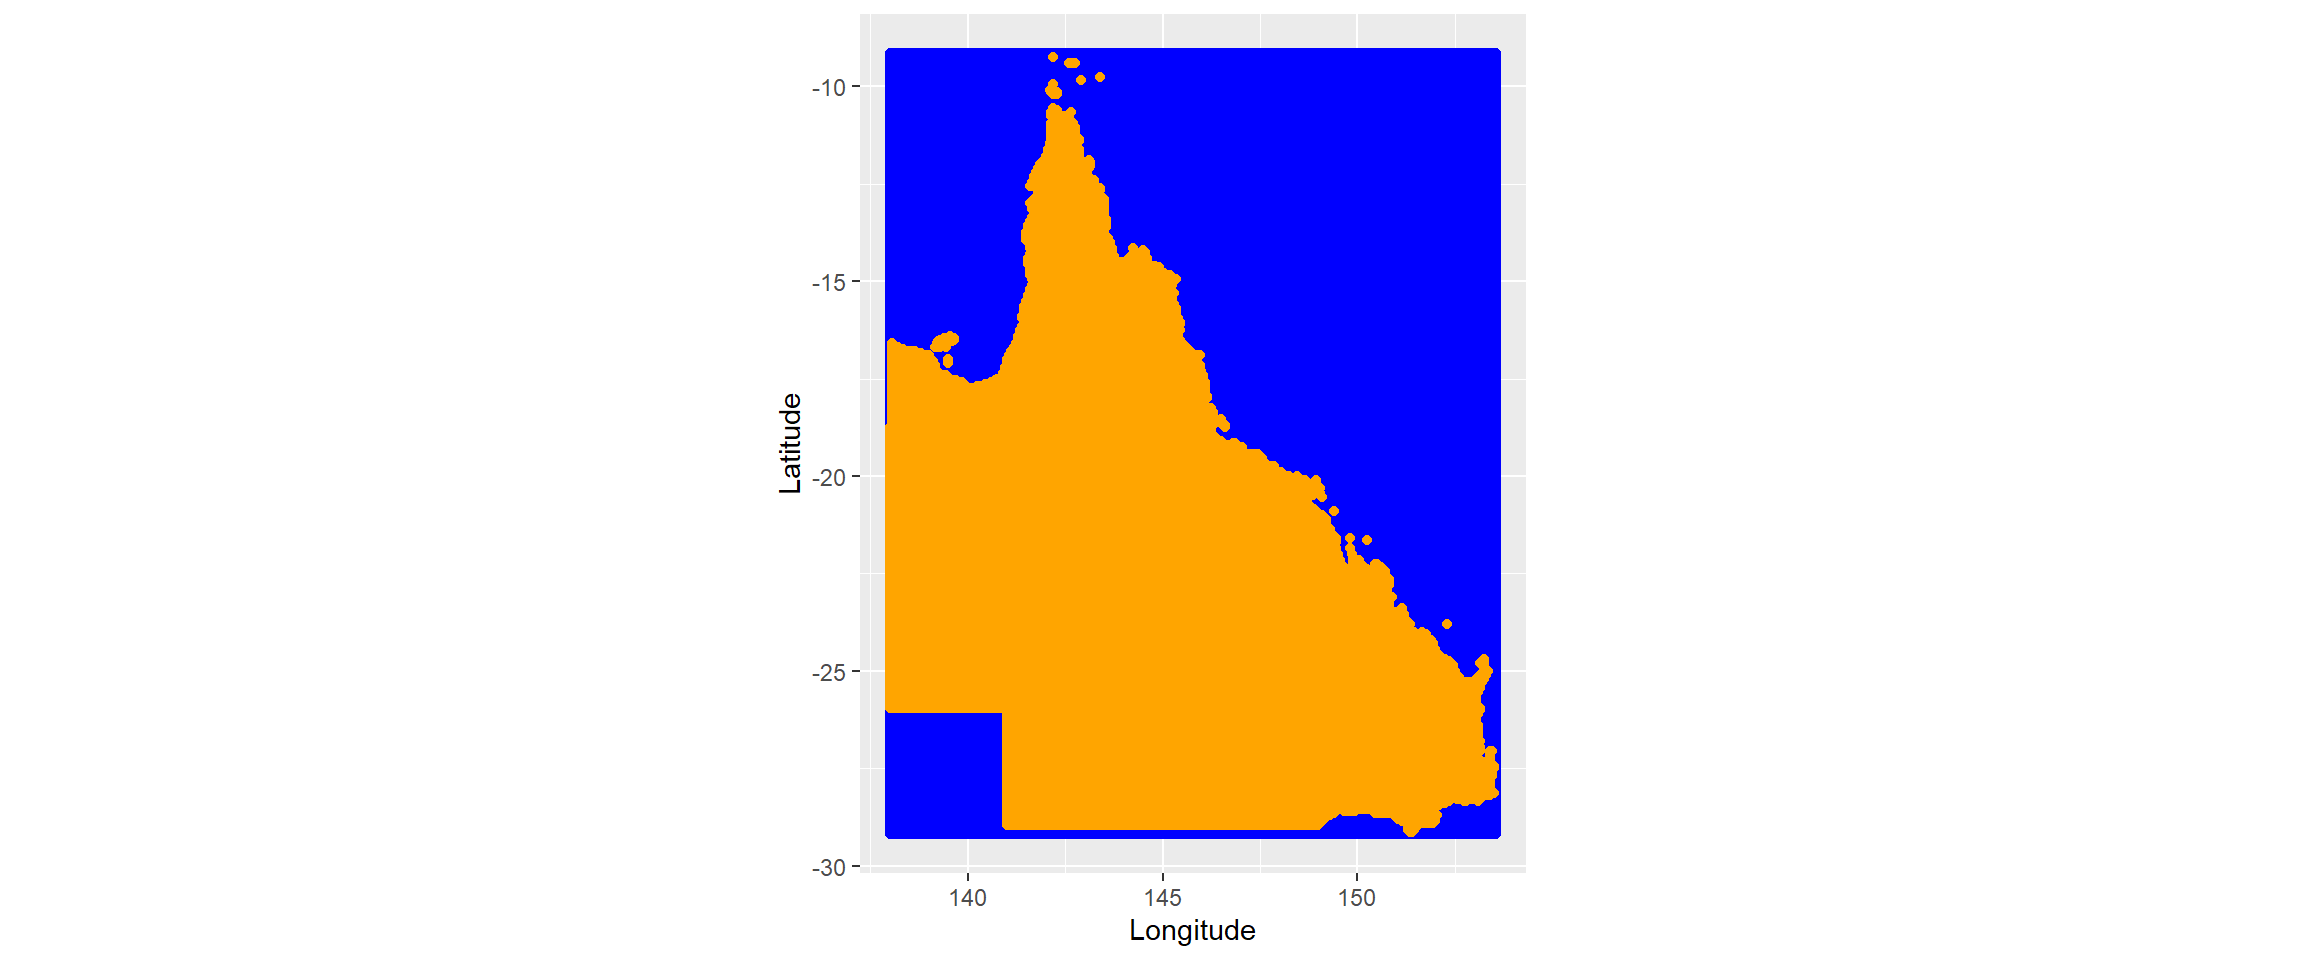
\includegraphics[width=1\linewidth]{interactive-maps_files/figure-latex/map-of-coord-grid-1} \caption{coordinates that we will use for kriging (initial grid in blue and those than intersect with QLD boundary in orange)}\label{fig:map-of-coord-grid}
\end{figure}

\hypertarget{kriging-finally}{%
\subsection{Kriging (finally)}\label{kriging-finally}}

Now we are ready to do the kriging. \texttt{gstat::krige()} requires that the \texttt{newdata} be of class \texttt{Spatial}, \texttt{sf}, or \texttt{stars}. Here, I specify the coordinates using \texttt{sp::coordinates()}. It also requires that you specify the variogram model within - here we use a circular model \texttt{vgm("Cir")} but there may be better choices for other data.

Figure \ref{fig:map-kriged-acute} shows the map with the interpolated values from kriging.

\begin{Shaded}
\begin{Highlighting}[]
\NormalTok{lzn\_vgm }\OtherTok{\textless{}{-}} \FunctionTok{variogram}\NormalTok{(time }\SpecialCharTok{\textasciitilde{}} \DecValTok{1}\NormalTok{, df\_towns)}
\NormalTok{lzn\_fit }\OtherTok{\textless{}{-}} \FunctionTok{fit.variogram}\NormalTok{(lzn\_vgm, }\AttributeTok{model=}\FunctionTok{vgm}\NormalTok{(}\StringTok{"Sph"}\NormalTok{))}

\FunctionTok{coordinates}\NormalTok{(pnts\_in\_qld) }\OtherTok{\textless{}{-}} \ErrorTok{\textasciitilde{}}\NormalTok{ X }\SpecialCharTok{+}\NormalTok{ Y}

\NormalTok{kriged\_layer }\OtherTok{\textless{}{-}}
  \FunctionTok{krige}\NormalTok{(}
    \AttributeTok{formula=}\NormalTok{time }\SpecialCharTok{\textasciitilde{}} \DecValTok{1}\NormalTok{, }
    \AttributeTok{locations=}\NormalTok{df\_towns,}
    \AttributeTok{newdata=}\NormalTok{pnts\_in\_qld,}
    \AttributeTok{model=}\NormalTok{lzn\_fit}
\NormalTok{  ) }\SpecialCharTok{\%\textgreater{}\%}
  \FunctionTok{as.data.frame}\NormalTok{()}
\end{Highlighting}
\end{Shaded}

\begin{verbatim}
## [using ordinary kriging]
\end{verbatim}

\begin{Shaded}
\begin{Highlighting}[]
\FunctionTok{ggplot}\NormalTok{(}\AttributeTok{data=}\NormalTok{kriged\_layer, }\FunctionTok{aes}\NormalTok{(X, Y, }\AttributeTok{col=}\NormalTok{var1.pred)) }\SpecialCharTok{+} 
  \FunctionTok{geom\_point}\NormalTok{() }\SpecialCharTok{+}
  \FunctionTok{scale\_colour\_gradientn}\NormalTok{(}\AttributeTok{colors=}\FunctionTok{c}\NormalTok{(}\StringTok{"yellow"}\NormalTok{, }\StringTok{"orange"}\NormalTok{, }\StringTok{"red"}\NormalTok{, }\StringTok{"black"}\NormalTok{)) }\SpecialCharTok{+}
  \FunctionTok{coord\_equal}\NormalTok{() }\SpecialCharTok{+}
  \FunctionTok{labs}\NormalTok{(}
    \AttributeTok{x=}\StringTok{"Longitude"}\NormalTok{,}
    \AttributeTok{y=}\StringTok{"Latitude"}
\NormalTok{  )}
\end{Highlighting}
\end{Shaded}

\begin{figure}
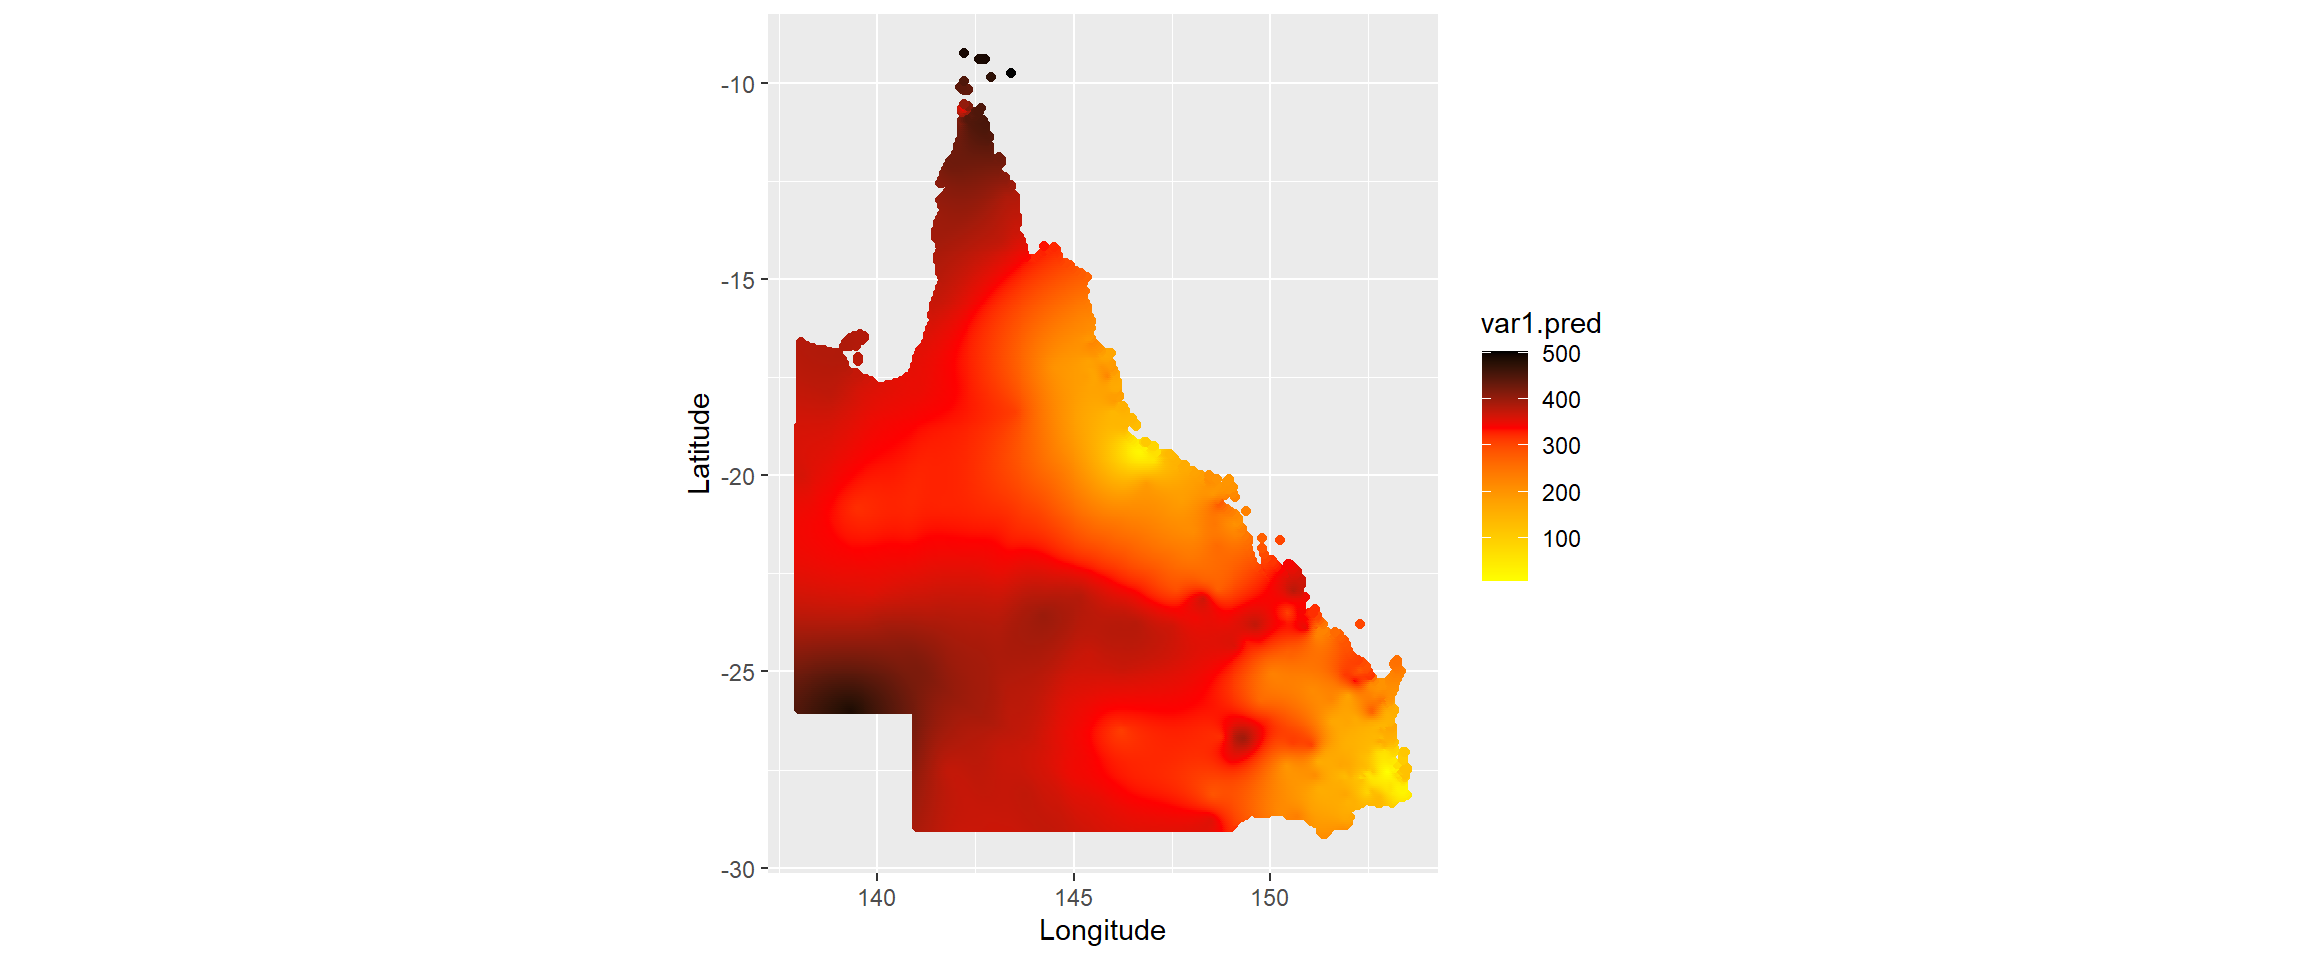
\includegraphics[width=1\linewidth]{interactive-maps_files/figure-latex/map-kriged-acute-1} \caption{coordinates that we will use for kriging (initial grid in blue and those than intersect with QLD boundary in orange)}\label{fig:map-kriged-acute}
\end{figure}

\hypertarget{making-rasters}{%
\subsection{Making rasters}\label{making-rasters}}

Now we can turn our grid of interpolated values into the rasters that we can then use in a leaflet map. We use the \texttt{raster} package. Figure \ref{leaflet-map-raster} shows our kriged output as a raster on a leaflet map, the same type of objects as what's used in iTRAQI.

\begin{Shaded}
\begin{Highlighting}[]
\NormalTok{raster\_layer }\OtherTok{\textless{}{-}}\NormalTok{ raster}\SpecialCharTok{::}\FunctionTok{rasterFromXYZ}\NormalTok{(kriged\_layer, }\AttributeTok{crs=}\DecValTok{4326}\NormalTok{, }\AttributeTok{res=}\FloatTok{0.05}\NormalTok{)}
\NormalTok{raster\_layer }\OtherTok{\textless{}{-}}\NormalTok{ raster}\SpecialCharTok{::}\FunctionTok{raster}\NormalTok{(raster\_layer, }\AttributeTok{layer=}\DecValTok{1}\NormalTok{) }\CommentTok{\# layer=1 to select the prediction values rather than the variance}

\FunctionTok{leaflet}\NormalTok{() }\SpecialCharTok{\%\textgreater{}\%}
  \FunctionTok{addProviderTiles}\NormalTok{(}\StringTok{"CartoDB.VoyagerNoLabels"}\NormalTok{) }\SpecialCharTok{\%\textgreater{}\%}
  \FunctionTok{addRasterImage}\NormalTok{(}\AttributeTok{x=}\NormalTok{raster\_layer, }\AttributeTok{colors=}\StringTok{"YlOrRd"}\NormalTok{)}
\end{Highlighting}
\end{Shaded}

\begin{figure}
\includegraphics[width=1\linewidth]{interactive-maps_files/figure-latex/leaflet-map-raster-1} \caption{coordinates that we will use for kriging (initial grid in blue and those than intersect with QLD boundary in orange)}\label{fig:leaflet-map-raster}
\end{figure}

\hypertarget{polygons}{%
\section{Polygons}\label{polygons}}

We are going to download our polygons from the Australian Bureau of Statistics.

The link to the downloads page for the 2016 Australian Statistical Geography Standard (ASGS) files are \href{https://www.abs.gov.au/AUSSTATS/abs@.nsf/DetailsPage/1270.0.55.001July\%202016?OpenDocument}{here} and the particular file that we are going to download is the `Queensland Mesh Blocks ASGS Ed 2016 Digital Boundaries in ESRI Shapefile Format'.
You will have to download the zipped file and unzip it somewhere locally. I've done so and saved it in the same directory as the other downloaded files and unzipped it into a folder there called `qld\_shape'. Having done that, I can import it using \texttt{st\_read()}

\begin{Shaded}
\begin{Highlighting}[]
\NormalTok{qld\_SAs2016 }\OtherTok{\textless{}{-}} \FunctionTok{st\_read}\NormalTok{(}\FunctionTok{file.path}\NormalTok{(save\_dir, }\StringTok{"qld\_shape/MB\_2016\_QLD.shp"}\NormalTok{))}
\end{Highlighting}
\end{Shaded}

\begin{verbatim}
## Reading layer `MB_2016_QLD' from data source 
##   `C:\Users\n10891277\OneDrive - Queensland University of Technology\Documents\R_projects\interactive-maps\input\qld_shape\MB_2016_QLD.shp' 
##   using driver `ESRI Shapefile'
## replacing null geometries with empty geometries
## Simple feature collection with 69764 features and 16 fields (with 25 geometries empty)
## Geometry type: POLYGON
## Dimension:     XY
## Bounding box:  xmin: 137.9943 ymin: -29.1779 xmax: 153.5522 ymax: -9.142176
## Geodetic CRS:  GDA94
\end{verbatim}

\begin{Shaded}
\begin{Highlighting}[]
\FunctionTok{head}\NormalTok{(qld\_SAs2016)}
\end{Highlighting}
\end{Shaded}

\begin{verbatim}
## Simple feature collection with 6 features and 16 fields (with 1 geometry empty)
## Geometry type: POLYGON
## Dimension:     XY
## Bounding box:  xmin: 144.5488 ymin: -22.97163 xmax: 147.0728 ymax: -19.24556
## Geodetic CRS:  GDA94
##     MB_CODE16         MB_CAT16  SA1_MAIN16 SA1_7DIG16 SA2_MAIN16 SA2_5DIG16
## 1 30000009499 NOUSUALRESIDENCE 39999949999    3949999  399999499      39499
## 2 30000010000         Parkland 31802148912    3148912  318021489      31489
## 3 30000020000         Parkland 31802148912    3148912  318021489      31489
## 4 30000030000         Parkland 31802148912    3148912  318021489      31489
## 5 30000050000      Residential 31503140809    3140809  315031408      31408
## 6 30000160000      Residential 31503140808    3140808  315031408      31408
##               SA2_NAME16 SA3_CODE16             SA3_NAME16 SA4_CODE16
## 1 No usual address (Qld)      39999 No usual address (Qld)        399
## 2     Townsville - South      31802             Townsville        318
## 3     Townsville - South      31802             Townsville        318
## 4     Townsville - South      31802             Townsville        318
## 5  Barcaldine - Blackall      31503        Outback - South        315
## 6  Barcaldine - Blackall      31503        Outback - South        315
##               SA4_NAME16 GCC_CODE16             GCC_NAME16 STE_CODE16
## 1 No usual address (Qld)      39499 No usual address (Qld)          3
## 2             Townsville      3RQLD            Rest of Qld          3
## 3             Townsville      3RQLD            Rest of Qld          3
## 4             Townsville      3RQLD            Rest of Qld          3
## 5   Queensland - Outback      3RQLD            Rest of Qld          3
## 6   Queensland - Outback      3RQLD            Rest of Qld          3
##   STE_NAME16 AREASQKM16                       geometry
## 1 Queensland     0.0000                  POLYGON EMPTY
## 2 Queensland     0.0387 POLYGON ((147.0641 -19.2466...
## 3 Queensland     0.0071 POLYGON ((147.0715 -19.2576...
## 4 Queensland     0.0004 POLYGON ((147.0615 -19.2460...
## 5 Queensland     0.0432 POLYGON ((145.2406 -22.9713...
## 6 Queensland     0.2156 POLYGON ((144.5493 -22.5902...
\end{verbatim}

This data has polygons for every Statistical Area level 1 (SA1) in Queensland but also details the SA2, SA3, and SA4 that that area is within. If we want to only use SA1's then we are fine to use the data here, but if we want to use these higher levels too, then we would either need (1) make a new object with dissolved boundaries within that higher level or (2) download more files from the ABS for those specific levels and filter to keep only Queensland. These files that we could use, say for SA2's are called `Statistical Area Level 2 (SA2) ASGS Ed 2016 Digital Boundaries in ESRI Shapefile Format', available at that same \href{https://www.abs.gov.au/AUSSTATS/abs@.nsf/DetailsPage/1270.0.55.001July\%202016?OpenDocument}{link}.

Since it's easy to filter, and reading this book is about learning new things (and my github repository is limited to 100mb), I'll show you the first approach that aggregates polygons within these higher levels.

Before we make a function to aggregate within different levels, I'm going to rename the columns in the object so that they're all named consistently - you may have noticed the unique identifier for SA1's is called `SA1\_MAIN16' whereas for SA3's it's called `SA3\_CODE16'. I prefer `CODE'.

\begin{Shaded}
\begin{Highlighting}[]
\NormalTok{qld\_SAs2016 }\OtherTok{\textless{}{-}}
  \FunctionTok{rename}\NormalTok{(qld\_SAs2016, }\AttributeTok{SA1\_CODE16=}\NormalTok{SA1\_MAIN16, }\AttributeTok{SA2\_CODE16=}\NormalTok{SA2\_MAIN16)}
\end{Highlighting}
\end{Shaded}

\hypertarget{dissolving-polygons-to-get-sa2s-and-sa3s}{%
\subsection{Dissolving polygons to get SA2s and SA3s}\label{dissolving-polygons-to-get-sa2s-and-sa3s}}

The function below will dissolve the boundaries for all the polygons within the SA-level that we pick. The work here is done by \texttt{rmapshaper::ms\_dissolve()}. I'll use this to make separate objects for SA2s and SA3s. Since this returns back only the geometry of the polygon and the name, I'll make the same change for my SA1s. By selecting only the code, I get the object with the code AND the geometry - unless I transform the object into a data.frame first, it will always keep the geometry.

\begin{Shaded}
\begin{Highlighting}[]
\NormalTok{aggregate\_by\_SA }\OtherTok{\textless{}{-}} \ControlFlowTok{function}\NormalTok{(qld\_sf, SA\_number)\{}
\NormalTok{  sa\_main }\OtherTok{\textless{}{-}}\NormalTok{ glue}\SpecialCharTok{::}\FunctionTok{glue}\NormalTok{(}\StringTok{\textquotesingle{}SA\{SA\_number\}\_CODE16\textquotesingle{}}\NormalTok{)}
  \ControlFlowTok{if}\NormalTok{(}\SpecialCharTok{!}\NormalTok{sa\_main }\SpecialCharTok{\%in\%} \FunctionTok{names}\NormalTok{(qld\_sf)) }\FunctionTok{return}\NormalTok{(}\FunctionTok{message}\NormalTok{(sa\_main, }\StringTok{" was not found in polygon layer"}\NormalTok{))}
  \FunctionTok{message}\NormalTok{(glue}\SpecialCharTok{::}\FunctionTok{glue}\NormalTok{(}\StringTok{\textquotesingle{}{-}{-}{-}{-}{-} grouping polygons within SA\{SA\_number\} {-}{-}{-}{-}{-}\textquotesingle{}}\NormalTok{))}
\NormalTok{  rmapshaper}\SpecialCharTok{::}\FunctionTok{ms\_dissolve}\NormalTok{(qld\_sf, sa\_main)}
\NormalTok{\}}


\NormalTok{qld\_SA2s }\OtherTok{\textless{}{-}} \FunctionTok{aggregate\_by\_SA}\NormalTok{(}\AttributeTok{qld\_sf=}\NormalTok{qld\_SAs2016, }\AttributeTok{SA\_number=}\DecValTok{2}\NormalTok{)}
\end{Highlighting}
\end{Shaded}

\begin{verbatim}
## ----- grouping polygons within SA2 -----
\end{verbatim}

\begin{verbatim}
## Registered S3 method overwritten by 'geojsonlint':
##   method         from 
##   print.location dplyr
\end{verbatim}

\begin{Shaded}
\begin{Highlighting}[]
\NormalTok{qld\_SA3s }\OtherTok{\textless{}{-}} \FunctionTok{aggregate\_by\_SA}\NormalTok{(}\AttributeTok{qld\_sf=}\NormalTok{qld\_SAs2016, }\AttributeTok{SA\_number=}\DecValTok{3}\NormalTok{)}
\end{Highlighting}
\end{Shaded}

\begin{verbatim}
## ----- grouping polygons within SA3 -----
\end{verbatim}

\begin{Shaded}
\begin{Highlighting}[]
\NormalTok{qld\_SA1s }\OtherTok{\textless{}{-}}\NormalTok{ qld\_SAs2016 }\SpecialCharTok{\%\textgreater{}\%} \FunctionTok{select}\NormalTok{(SA1\_CODE16)}
\FunctionTok{head}\NormalTok{(qld\_SA1s)}
\end{Highlighting}
\end{Shaded}

\begin{verbatim}
## Simple feature collection with 6 features and 1 field (with 1 geometry empty)
## Geometry type: POLYGON
## Dimension:     XY
## Bounding box:  xmin: 144.5488 ymin: -22.97163 xmax: 147.0728 ymax: -19.24556
## Geodetic CRS:  GDA94
##    SA1_CODE16                       geometry
## 1 39999949999                  POLYGON EMPTY
## 2 31802148912 POLYGON ((147.0641 -19.2466...
## 3 31802148912 POLYGON ((147.0715 -19.2576...
## 4 31802148912 POLYGON ((147.0615 -19.2460...
## 5 31503140809 POLYGON ((145.2406 -22.9713...
## 6 31503140808 POLYGON ((144.5493 -22.5902...
\end{verbatim}

\begin{Shaded}
\begin{Highlighting}[]
\FunctionTok{head}\NormalTok{(qld\_SA2s)}
\end{Highlighting}
\end{Shaded}

\begin{verbatim}
## Simple feature collection with 6 features and 1 field (with 1 geometry empty)
## Geometry type: GEOMETRY
## Dimension:     XY
## Bounding box:  xmin: 141.4665 ymin: -25.75471 xmax: 147.2964 ymax: -12.56014
## Geodetic CRS:  GDA94
##   SA2_CODE16                       geometry
## 1  399999499             MULTIPOLYGON EMPTY
## 2  318021489 MULTIPOLYGON (((147.0641 -1...
## 3  315031408 POLYGON ((143.6141 -22.5387...
## 4  306051166 POLYGON ((145.4269 -17.1212...
## 5  306051169 POLYGON ((145.5535 -17.1354...
## 6  315011395 MULTIPOLYGON (((141.765 -12...
\end{verbatim}

There are some empty geometries here, so we find (and then remove) these using \texttt{st\_is\_empty()}.

\begin{Shaded}
\begin{Highlighting}[]
\NormalTok{qld\_SA1s }\OtherTok{\textless{}{-}}\NormalTok{ qld\_SA1s[}\SpecialCharTok{!}\FunctionTok{st\_is\_empty}\NormalTok{(qld\_SA1s), , drop}\OtherTok{=}\ConstantTok{FALSE}\NormalTok{]}
\NormalTok{qld\_SA2s }\OtherTok{\textless{}{-}}\NormalTok{ qld\_SA2s[}\SpecialCharTok{!}\FunctionTok{st\_is\_empty}\NormalTok{(qld\_SA2s), , drop}\OtherTok{=}\ConstantTok{FALSE}\NormalTok{]}
\NormalTok{qld\_SA3s }\OtherTok{\textless{}{-}}\NormalTok{ qld\_SA3s[}\SpecialCharTok{!}\FunctionTok{st\_is\_empty}\NormalTok{(qld\_SA3s), , drop}\OtherTok{=}\ConstantTok{FALSE}\NormalTok{]}
\end{Highlighting}
\end{Shaded}

Run the code to become impatient and find out how long it takes leaflet to display such a detailed polygon layer.

\begin{Shaded}
\begin{Highlighting}[]
\FunctionTok{leaflet}\NormalTok{() }\SpecialCharTok{\%\textgreater{}\%}
  \FunctionTok{addTiles}\NormalTok{() }\SpecialCharTok{\%\textgreater{}\%}
  \FunctionTok{addPolygons}\NormalTok{(}
    \AttributeTok{data=}\NormalTok{qld\_SA1s,}
    \AttributeTok{fillColor=}\StringTok{"Orange"}\NormalTok{,}
    \AttributeTok{color=}\StringTok{"black"}\NormalTok{,}
    \AttributeTok{weight=}\DecValTok{1}
\NormalTok{  )}
\end{Highlighting}
\end{Shaded}

\hypertarget{simplifying-polygons-to-reduce-rendering-time-with-leaflet}{%
\subsection{Simplifying polygons to reduce rendering time with leaflet}\label{simplifying-polygons-to-reduce-rendering-time-with-leaflet}}

We need to do something about this - fortunately, we don't need all the incredible amounts of detail in the polygons for our map, so we can simplify them using \texttt{rmapshaper::ms\_simplify()}.
Simplifying the polygons can take a few minutes but it makes the maps much faster to display.

\begin{Shaded}
\begin{Highlighting}[]
\NormalTok{qld\_SA1s }\OtherTok{\textless{}{-}}\NormalTok{ rmapshaper}\SpecialCharTok{::}\FunctionTok{ms\_simplify}\NormalTok{(qld\_SA1s, }\AttributeTok{keep=}\FloatTok{0.03}\NormalTok{)}
\NormalTok{qld\_SA2s }\OtherTok{\textless{}{-}}\NormalTok{ rmapshaper}\SpecialCharTok{::}\FunctionTok{ms\_simplify}\NormalTok{(qld\_SA2s, }\AttributeTok{keep=}\FloatTok{0.03}\NormalTok{)}
\NormalTok{qld\_SA3s }\OtherTok{\textless{}{-}}\NormalTok{ rmapshaper}\SpecialCharTok{::}\FunctionTok{ms\_simplify}\NormalTok{(qld\_SA3s, }\AttributeTok{keep=}\FloatTok{0.03}\NormalTok{)}

\FunctionTok{leaflet}\NormalTok{() }\SpecialCharTok{\%\textgreater{}\%}
  \FunctionTok{addTiles}\NormalTok{() }\SpecialCharTok{\%\textgreater{}\%}
  \FunctionTok{addPolygons}\NormalTok{(}
    \AttributeTok{data=}\NormalTok{qld\_SA1s,}
    \AttributeTok{fillColor=}\StringTok{"yellow"}\NormalTok{,}
    \AttributeTok{color=}\StringTok{"black"}\NormalTok{,}
    \AttributeTok{weight=}\DecValTok{1}\NormalTok{,}
    \AttributeTok{group=}\StringTok{"SA1"}
\NormalTok{  ) }\SpecialCharTok{\%\textgreater{}\%}
  \FunctionTok{addPolygons}\NormalTok{(}
    \AttributeTok{data=}\NormalTok{qld\_SA2s,}
    \AttributeTok{fillColor=}\StringTok{"orange"}\NormalTok{,}
    \AttributeTok{color=}\StringTok{"black"}\NormalTok{,}
    \AttributeTok{weight=}\DecValTok{1}\NormalTok{,}
    \AttributeTok{group=}\StringTok{"SA2"}
\NormalTok{  ) }\SpecialCharTok{\%\textgreater{}\%}
  \FunctionTok{addPolygons}\NormalTok{(}
    \AttributeTok{data=}\NormalTok{qld\_SA3s,}
    \AttributeTok{fillColor=}\StringTok{"red"}\NormalTok{,}
    \AttributeTok{color=}\StringTok{"black"}\NormalTok{,}
    \AttributeTok{weight=}\DecValTok{1}\NormalTok{,}
    \AttributeTok{group=}\StringTok{"SA3"}
\NormalTok{  ) }\SpecialCharTok{\%\textgreater{}\%}
  \FunctionTok{addLayersControl}\NormalTok{(}
    \AttributeTok{position=}\StringTok{"topright"}\NormalTok{,}
    \AttributeTok{baseGroups=}\FunctionTok{c}\NormalTok{(}\StringTok{"SA1"}\NormalTok{, }\StringTok{"SA2"}\NormalTok{, }\StringTok{"SA3"}\NormalTok{),}
    \AttributeTok{options=}\FunctionTok{layersControlOptions}\NormalTok{(}\AttributeTok{collapsed =} \ConstantTok{FALSE}\NormalTok{)}
\NormalTok{  )}
\end{Highlighting}
\end{Shaded}

\includegraphics{interactive-maps_files/figure-latex/simplify-polygons-1.pdf}

\hypertarget{spatial-joins-and-aggregations}{%
\subsection{Spatial joins and aggregations}\label{spatial-joins-and-aggregations}}

To get estimates and ranges for travel times within each SA1 and SA2 for iTRAQI, we aggregated the interpolated values within those polygons. To do this, we need to first (1) join the data that we made from kriging to the polygons data, and (2) aggregate the values within those areas to calculate the summary statistics that we want to show.

Here is the data that we made from kriging previously.

\begin{Shaded}
\begin{Highlighting}[]
\FunctionTok{head}\NormalTok{(}\FunctionTok{select}\NormalTok{(kriged\_layer, }\SpecialCharTok{{-}}\NormalTok{var1.var), }\DecValTok{5}\NormalTok{)}
\end{Highlighting}
\end{Shaded}

\begin{verbatim}
##        X      Y var1.pred
## 1 151.35 -29.15  204.9349
## 2 151.40 -29.15  204.0813
## 3 151.30 -29.10  203.9246
## 4 151.35 -29.10  202.9899
## 5 151.40 -29.10  202.1970
\end{verbatim}

\hypertarget{joins}{%
\subsubsection{Joins}\label{joins}}

We do this join using \texttt{sf::st\_join()} but this requires that both the sf objects for the polygons and the kriging points share the same coordinates system. First, we need to make our kriging data into a spatial data.frame then set the coordinate reference system (crs) to match. The polygons that we downloaded from the ABS used the GDA94 reference system and this can be matched to \href{https://epsg.io/4283}{EPSG:4283 online}.

\begin{Shaded}
\begin{Highlighting}[]
\NormalTok{kriged\_df }\OtherTok{\textless{}{-}}\NormalTok{ kriged\_layer }\SpecialCharTok{\%\textgreater{}\%} \FunctionTok{select}\NormalTok{(}\SpecialCharTok{{-}}\NormalTok{var1.var)}
\FunctionTok{coordinates}\NormalTok{(kriged\_df) }\OtherTok{\textless{}{-}} \ErrorTok{\textasciitilde{}}\NormalTok{ X }\SpecialCharTok{+}\NormalTok{ Y}
\NormalTok{kriged\_sf }\OtherTok{\textless{}{-}} \FunctionTok{st\_as\_sf}\NormalTok{(kriged\_df)}
\NormalTok{kriged\_sf }\OtherTok{\textless{}{-}} \FunctionTok{st\_set\_crs}\NormalTok{(kriged\_sf, }\DecValTok{4283}\NormalTok{)}
\end{Highlighting}
\end{Shaded}

Having asigned the appropriate crs, we can use \texttt{st\_join} (if the crs of both objects isn't the same, \texttt{st\_join} will throw an error).

Now the resulting object has about the same number of features (rows) as we had in the interpolation data

\begin{Shaded}
\begin{Highlighting}[]
\NormalTok{qld\_SA3s\_joined }\OtherTok{\textless{}{-}} \FunctionTok{st\_join}\NormalTok{(qld\_SA3s, kriged\_sf)}
\FunctionTok{head}\NormalTok{(qld\_SA3s\_joined)}
\end{Highlighting}
\end{Shaded}

\begin{verbatim}
## Simple feature collection with 6 features and 2 fields
## Geometry type: MULTIPOLYGON
## Dimension:     XY
## Bounding box:  xmin: 146.1469 ymin: -19.7847 xmax: 147.1202 ymax: -18.92276
## Geodetic CRS:  GDA94
##     SA3_CODE16 var1.pred                       geometry
## 1        31802  79.97241 MULTIPOLYGON (((146.3237 -1...
## 1.1      31802  81.29616 MULTIPOLYGON (((146.3237 -1...
## 1.2      31802  83.43087 MULTIPOLYGON (((146.3237 -1...
## 1.3      31802  71.45434 MULTIPOLYGON (((146.3237 -1...
## 1.4      31802  70.50484 MULTIPOLYGON (((146.3237 -1...
## 1.5      31802  70.27281 MULTIPOLYGON (((146.3237 -1...
\end{verbatim}

\begin{Shaded}
\begin{Highlighting}[]
\FunctionTok{nrow}\NormalTok{(qld\_SA3s\_joined)}
\end{Highlighting}
\end{Shaded}

\begin{verbatim}
## [1] 60863
\end{verbatim}

\begin{Shaded}
\begin{Highlighting}[]
\FunctionTok{nrow}\NormalTok{(kriged\_df)}
\end{Highlighting}
\end{Shaded}

\begin{verbatim}
## [1] 60888
\end{verbatim}

\hypertarget{aggregations}{%
\subsubsection{Aggregations}\label{aggregations}}

If you're familiar with the \texttt{dplyr::} ways of grouping and aggregating, then this step will be familiar to working with data.frames. To this larger dataset within the unique polygons, we use \texttt{group\_by} and \texttt{summarise}. Here, we will get the minimum, maximum, and median of the predicted values.

\begin{Shaded}
\begin{Highlighting}[]
\NormalTok{qld\_SA3s\_aggregated }\OtherTok{\textless{}{-}} 
\NormalTok{  qld\_SA3s\_joined }\SpecialCharTok{\%\textgreater{}\%}
  \FunctionTok{group\_by}\NormalTok{(SA3\_CODE16) }\SpecialCharTok{\%\textgreater{}\%}
  \FunctionTok{summarize}\NormalTok{(}
    \AttributeTok{min=}\FunctionTok{min}\NormalTok{(var1.pred),}
    \AttributeTok{max=}\FunctionTok{max}\NormalTok{(var1.pred),}
    \AttributeTok{median=}\FunctionTok{median}\NormalTok{(var1.pred)}
\NormalTok{  )}
\end{Highlighting}
\end{Shaded}

Unfortunately, this is incredibly slow for some reason! It's much faster to take the data out from the sf object, do the aggregations and then join it back to the original sf object before we did the join.

\begin{Shaded}
\begin{Highlighting}[]
\NormalTok{qld\_SA3s\_joined\_df }\OtherTok{\textless{}{-}} \FunctionTok{as.data.frame}\NormalTok{(qld\_SA3s\_joined) }\SpecialCharTok{\%\textgreater{}\%} \FunctionTok{select}\NormalTok{(}\SpecialCharTok{{-}}\NormalTok{geometry)}

\NormalTok{qld\_SA3s\_aggregated\_df }\OtherTok{\textless{}{-}} 
\NormalTok{  qld\_SA3s\_joined\_df }\SpecialCharTok{\%\textgreater{}\%}
  \FunctionTok{group\_by}\NormalTok{(SA3\_CODE16) }\SpecialCharTok{\%\textgreater{}\%}
  \FunctionTok{summarize}\NormalTok{(}
    \AttributeTok{min=}\FunctionTok{min}\NormalTok{(var1.pred),}
    \AttributeTok{max=}\FunctionTok{max}\NormalTok{(var1.pred),}
    \AttributeTok{median=}\FunctionTok{median}\NormalTok{(var1.pred)}
\NormalTok{  )}

\NormalTok{qld\_SA3s\_aggregated }\OtherTok{\textless{}{-}} \FunctionTok{left\_join}\NormalTok{(qld\_SA3s, qld\_SA3s\_aggregated\_df, }\AttributeTok{by=}\StringTok{"SA3\_CODE16"}\NormalTok{) }
\end{Highlighting}
\end{Shaded}

To check that these aggregations look right, lets make a map to visualise the medians across different SA3s.

\begin{Shaded}
\begin{Highlighting}[]
\NormalTok{fill\_value }\OtherTok{\textless{}{-}}\NormalTok{ qld\_SA3s\_aggregated}\SpecialCharTok{$}\NormalTok{median}
\NormalTok{pal }\OtherTok{\textless{}{-}} \FunctionTok{colorNumeric}\NormalTok{(}\StringTok{"YlOrRd"}\NormalTok{, }\AttributeTok{domain=}\NormalTok{fill\_value)}

\FunctionTok{leaflet}\NormalTok{() }\SpecialCharTok{\%\textgreater{}\%}
  \FunctionTok{addTiles}\NormalTok{() }\SpecialCharTok{\%\textgreater{}\%}
  \FunctionTok{addPolygons}\NormalTok{(}
    \AttributeTok{data=}\NormalTok{qld\_SA3s\_aggregated,}
    \AttributeTok{fillColor=}\FunctionTok{pal}\NormalTok{(qld\_SA3s\_aggregated}\SpecialCharTok{$}\NormalTok{median),}
    \AttributeTok{color=}\StringTok{"black"}\NormalTok{,}
    \AttributeTok{weight=}\DecValTok{1}\NormalTok{,}
    \AttributeTok{fillOpacity=}\FloatTok{0.8}
\NormalTok{  )}
\end{Highlighting}
\end{Shaded}

\includegraphics{interactive-maps_files/figure-latex/aggregate-plot-1-1.pdf}

Looks good\ldots{} except?

\begin{Shaded}
\begin{Highlighting}[]
\FunctionTok{leaflet}\NormalTok{() }\SpecialCharTok{\%\textgreater{}\%}
  \FunctionTok{addTiles}\NormalTok{() }\SpecialCharTok{\%\textgreater{}\%}
  \FunctionTok{addPolygons}\NormalTok{(}
    \AttributeTok{data=}\NormalTok{qld\_SA3s\_aggregated,}
    \AttributeTok{fillColor=}\FunctionTok{pal}\NormalTok{(qld\_SA3s\_aggregated}\SpecialCharTok{$}\NormalTok{median),}
    \AttributeTok{color=}\StringTok{"black"}\NormalTok{,}
    \AttributeTok{weight=}\DecValTok{1}\NormalTok{,}
    \AttributeTok{fillOpacity=}\FloatTok{0.8}
\NormalTok{  ) }\SpecialCharTok{\%\textgreater{}\%}
  \FunctionTok{setView}\NormalTok{(}\FloatTok{153.026358}\NormalTok{, }\SpecialCharTok{{-}}\FloatTok{27.468562}\NormalTok{, }\AttributeTok{zoom=}\DecValTok{11}\NormalTok{)}
\end{Highlighting}
\end{Shaded}

\includegraphics{interactive-maps_files/figure-latex/aggregate-plot-2-1.pdf}

There's a section which is greyed out - this means that the aggregations returned \texttt{NA}.

Let's plot the coordinates which we have interpolated values for over the top.

\begin{Shaded}
\begin{Highlighting}[]
\NormalTok{kriged\_coordinates }\OtherTok{\textless{}{-}}
  \FunctionTok{as.data.frame}\NormalTok{(}\FunctionTok{coordinates}\NormalTok{(kriged\_df)) }\SpecialCharTok{\%\textgreater{}\%} 
  \FunctionTok{filter}\NormalTok{(X }\SpecialCharTok{\textless{}} \FloatTok{153.5}\NormalTok{, X }\SpecialCharTok{\textgreater{}} \FloatTok{152.3}\NormalTok{, Y }\SpecialCharTok{\textless{}} \SpecialCharTok{{-}}\DecValTok{27}\NormalTok{, Y }\SpecialCharTok{\textgreater{}} \SpecialCharTok{{-}}\DecValTok{28}\NormalTok{)}

\FunctionTok{leaflet}\NormalTok{() }\SpecialCharTok{\%\textgreater{}\%}
  \FunctionTok{addTiles}\NormalTok{() }\SpecialCharTok{\%\textgreater{}\%}
  \FunctionTok{addPolygons}\NormalTok{(}
    \AttributeTok{data=}\NormalTok{qld\_SA3s\_aggregated,}
    \AttributeTok{fillColor=}\FunctionTok{pal}\NormalTok{(qld\_SA3s\_aggregated}\SpecialCharTok{$}\NormalTok{median),}
    \AttributeTok{color=}\StringTok{"black"}\NormalTok{,}
    \AttributeTok{weight=}\DecValTok{1}\NormalTok{,}
    \AttributeTok{fillOpacity=}\FloatTok{0.8}
\NormalTok{  ) }\SpecialCharTok{\%\textgreater{}\%}
  \FunctionTok{setView}\NormalTok{(}\FloatTok{153.026358}\NormalTok{, }\SpecialCharTok{{-}}\FloatTok{27.468562}\NormalTok{, }\AttributeTok{zoom=}\DecValTok{11}\NormalTok{) }\SpecialCharTok{\%\textgreater{}\%}
  \FunctionTok{addCircleMarkers}\NormalTok{(}
    \AttributeTok{lng=}\NormalTok{kriged\_coordinates}\SpecialCharTok{$}\NormalTok{X, }
    \AttributeTok{lat=}\NormalTok{kriged\_coordinates}\SpecialCharTok{$}\NormalTok{Y,}
    \AttributeTok{radius=}\FloatTok{0.2}
\NormalTok{  )}
\end{Highlighting}
\end{Shaded}

\includegraphics{interactive-maps_files/figure-latex/aggregate-plot-3-1.pdf}

Looks like we missed the target with our the coordinates that we have interpolations for!

\includegraphics[width=3.125in,height=\textheight]{www/a-ha.gif}

There was a little primer to this problem when introducing the for kriging grid.
There are a couple solutions to this (that I can think of):

\begin{itemize}
\tightlist
\item
  Do a ludicrously granular grid for kriging so that we almost certainly have a point within every polygon, say every 50 square meters.
\item
  We add some points to the grid for kriging so that we ensure that we have at least 1 or more points within each polygon.
\end{itemize}

For iTRAQI, we did the latter. SA1s can be pretty small, so I don't want to have to keep trying smaller and smaller cell sizes for the kriging grid until I don't get any NA's. It's easier (and a lot faster) to get the centroid (coordinate for the centre) of every polygon and append this to the grid we use for kriging.

You can get the centroid of each polygon by using \texttt{sf::st\_centroid()} and the coordinates out of this object with \texttt{sf::st\_coordinates()}.

In the map below, we get these centroids and add them as additional coordinates to the map in red.

\begin{Shaded}
\begin{Highlighting}[]
\NormalTok{centroids }\OtherTok{\textless{}{-}} \FunctionTok{st\_centroid}\NormalTok{(qld\_SA3s, }\AttributeTok{of\_largest\_polygon=}\ConstantTok{TRUE}\NormalTok{)}
\NormalTok{centroid\_coords }\OtherTok{\textless{}{-}} \FunctionTok{as.data.frame}\NormalTok{(}\FunctionTok{st\_coordinates}\NormalTok{(centroids))}

\FunctionTok{leaflet}\NormalTok{() }\SpecialCharTok{\%\textgreater{}\%}
  \FunctionTok{addTiles}\NormalTok{() }\SpecialCharTok{\%\textgreater{}\%}
  \FunctionTok{addPolygons}\NormalTok{(}
    \AttributeTok{data=}\NormalTok{qld\_SA3s\_aggregated,}
    \AttributeTok{fillColor=}\FunctionTok{pal}\NormalTok{(qld\_SA3s\_aggregated}\SpecialCharTok{$}\NormalTok{median),}
    \AttributeTok{color=}\StringTok{"black"}\NormalTok{,}
    \AttributeTok{weight=}\DecValTok{1}\NormalTok{,}
    \AttributeTok{fillOpacity=}\FloatTok{0.8}
\NormalTok{  ) }\SpecialCharTok{\%\textgreater{}\%}
  \FunctionTok{setView}\NormalTok{(}\FloatTok{153.026358}\NormalTok{, }\SpecialCharTok{{-}}\FloatTok{27.468562}\NormalTok{, }\AttributeTok{zoom=}\DecValTok{11}\NormalTok{) }\SpecialCharTok{\%\textgreater{}\%}
  \FunctionTok{addCircleMarkers}\NormalTok{(}
    \AttributeTok{lng=}\NormalTok{kriged\_coordinates}\SpecialCharTok{$}\NormalTok{X, }
    \AttributeTok{lat=}\NormalTok{kriged\_coordinates}\SpecialCharTok{$}\NormalTok{Y,}
    \AttributeTok{radius=}\FloatTok{0.2}
\NormalTok{  ) }\SpecialCharTok{\%\textgreater{}\%}
  \FunctionTok{addCircleMarkers}\NormalTok{(}
    \AttributeTok{lng=}\NormalTok{centroid\_coords}\SpecialCharTok{$}\NormalTok{X, }
    \AttributeTok{lat=}\NormalTok{centroid\_coords}\SpecialCharTok{$}\NormalTok{Y,}
    \AttributeTok{color=}\StringTok{"red"}\NormalTok{,}
    \AttributeTok{radius=}\FloatTok{0.2}
\NormalTok{  )}
\end{Highlighting}
\end{Shaded}

\includegraphics{interactive-maps_files/figure-latex/aggregate-plot-4-1.pdf}

They're on target! The remaining steps would be to append this to the grid used for kriging, repeat the spatial join and aggregate within polygons.

However, I'm going to skip these steps and get straight into the shiny app development using the polygons that I've already made for iTRAQI.

\hypertarget{shiny-intro}{%
\chapter{An app with a map}\label{shiny-intro}}

This chapter will have a brief intro to shiny with a map:

\begin{itemize}
\tightlist
\item
  ui and server
\item
  reactivity
\item
  leaflet
\item
  leafletproxy
\end{itemize}

\hypertarget{a-bare-bones-shiny-app}{%
\section{A bare bones shiny app}\label{a-bare-bones-shiny-app}}

The most basic shiny app has a user-interface (\texttt{ui}) and a back-end (\texttt{server}) side. We control what content appears where on within the ui, and we control all the clever interactivity and generated content on the server side.

\begin{Shaded}
\begin{Highlighting}[]
\FunctionTok{library}\NormalTok{(shiny)}

\NormalTok{ui }\OtherTok{\textless{}{-}} \FunctionTok{fluidPage}\NormalTok{(}
  
\NormalTok{)}

\NormalTok{server }\OtherTok{\textless{}{-}} \ControlFlowTok{function}\NormalTok{(input, output, session) \{}
  
\NormalTok{\}}

\FunctionTok{shinyApp}\NormalTok{(ui, server)}
\end{Highlighting}
\end{Shaded}

This book will include many example shiny apps and accompanying code. However, since it'd be very time consuming to host all those apps independently, I will instead provide the code and sometimes an image of how the app displays. With every example app there will be a followup line of code with \texttt{shiny::runGitHub(...)} that you can use to run the app locally. If you run this line in R on your own computer, it will run the app in a way that you can then interact with it.

The inputs on the ui side always have an inputId and it is by this name that we access those values from the server. In the code below, we name an input as `n' and we access it in the server by calling \texttt{input\$n}. By accessing this input in such as way, within the expression used for \texttt{renderPlot()}, we are are asking the server side to update the plot every time that any inputs (\texttt{input\$\_\_\_}) used within it are updated.

\begin{Shaded}
\begin{Highlighting}[]
\FunctionTok{library}\NormalTok{(shiny)}

\NormalTok{ui }\OtherTok{\textless{}{-}} \FunctionTok{fluidPage}\NormalTok{(}
  \FunctionTok{numericInput}\NormalTok{(}\AttributeTok{inputId=}\StringTok{\textquotesingle{}n\textquotesingle{}}\NormalTok{, }\AttributeTok{label=}\StringTok{\textquotesingle{}sample size\textquotesingle{}}\NormalTok{, }\AttributeTok{value=}\DecValTok{10}\NormalTok{),}
  \FunctionTok{plotOutput}\NormalTok{(}\StringTok{\textquotesingle{}plot\textquotesingle{}}\NormalTok{)}
\NormalTok{)}

\NormalTok{server }\OtherTok{\textless{}{-}} \ControlFlowTok{function}\NormalTok{(input, output, session) \{}
\NormalTok{  output}\SpecialCharTok{$}\NormalTok{plot }\OtherTok{\textless{}{-}} \FunctionTok{renderPlot}\NormalTok{(}\AttributeTok{expr=}\NormalTok{\{}
    \FunctionTok{hist}\NormalTok{(}\AttributeTok{x=}\FunctionTok{rnorm}\NormalTok{(input}\SpecialCharTok{$}\NormalTok{n))}
\NormalTok{  \})}
\NormalTok{\}}

\FunctionTok{shinyApp}\NormalTok{(ui, server)}
\end{Highlighting}
\end{Shaded}

\begin{verbatim}
## 
## Listening on http://127.0.0.1:3992
\end{verbatim}

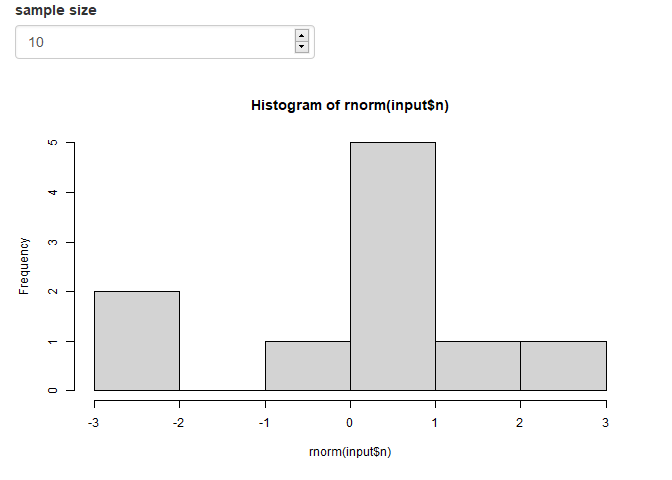
\includegraphics{interactive-maps_files/figure-latex/01-example-app-1.pdf}

(And here's your code to run the app locally)

\begin{Shaded}
\begin{Highlighting}[]
\NormalTok{shiny}\SpecialCharTok{::}\FunctionTok{runGitHub}\NormalTok{(}\StringTok{"RWParsons/interactive{-}maps"}\NormalTok{, }\AttributeTok{subdir=}\StringTok{"input/apps/01{-}example{-}app/"}\NormalTok{)}
\end{Highlighting}
\end{Shaded}

\hypertarget{leaflet-maps-in-shiny}{%
\section{Leaflet maps in shiny}\label{leaflet-maps-in-shiny}}

We're not here to make histograms, we're here to make maps!
I prefer the navigation between tabs (which you may want later) using \texttt{navbarPage} to design my ui.
These pages contain many panels that you can navigate between. Here's an app with a single \texttt{tabPanel} which contains our map.

\begin{Shaded}
\begin{Highlighting}[]
\FunctionTok{library}\NormalTok{(shiny)}
\FunctionTok{library}\NormalTok{(leaflet)}
\FunctionTok{library}\NormalTok{(tidyverse)}
\FunctionTok{library}\NormalTok{(sf)}
\NormalTok{input\_dir }\OtherTok{\textless{}{-}} \StringTok{"./input"}

\NormalTok{sa2\_polygons }\OtherTok{\textless{}{-}} \FunctionTok{readRDS}\NormalTok{(}\FunctionTok{file.path}\NormalTok{(input\_dir, }\StringTok{"stacked\_SA1\_and\_SA2\_polygons\_year2016\_simplified.rds"}\NormalTok{)) }\SpecialCharTok{\%\textgreater{}\%}
  \FunctionTok{filter}\NormalTok{(SA\_level}\SpecialCharTok{==}\DecValTok{2}\NormalTok{)}

\NormalTok{ui }\OtherTok{\textless{}{-}} \FunctionTok{navbarPage}\NormalTok{(}
  \StringTok{"App{-}with{-}a{-}map"}\NormalTok{, }\AttributeTok{id=}\StringTok{"nav"}\NormalTok{,}
  \FunctionTok{tabPanel}\NormalTok{(}
    \StringTok{"Map"}\NormalTok{,}
    \FunctionTok{leafletOutput}\NormalTok{(}\StringTok{\textquotesingle{}map\textquotesingle{}}\NormalTok{)}
\NormalTok{  )}
\NormalTok{)}

\NormalTok{server }\OtherTok{\textless{}{-}} \ControlFlowTok{function}\NormalTok{(input, output, session) \{}
\NormalTok{  output}\SpecialCharTok{$}\NormalTok{map }\OtherTok{\textless{}{-}} \FunctionTok{renderLeaflet}\NormalTok{(\{}
    \FunctionTok{leaflet}\NormalTok{() }\SpecialCharTok{\%\textgreater{}\%}
      \FunctionTok{addTiles}\NormalTok{() }\SpecialCharTok{\%\textgreater{}\%}
      \FunctionTok{addPolygons}\NormalTok{(}
        \AttributeTok{data=}\NormalTok{sa2\_polygons,}
        \AttributeTok{fillColor=}\StringTok{"Orange"}\NormalTok{,}
        \AttributeTok{color=}\StringTok{"black"}\NormalTok{,}
        \AttributeTok{weight=}\DecValTok{1}\NormalTok{,}
        \AttributeTok{group=}\StringTok{"Polygons"}
\NormalTok{      )}
\NormalTok{  \})}
\NormalTok{\}}

\FunctionTok{shinyApp}\NormalTok{(ui, server)}
\end{Highlighting}
\end{Shaded}

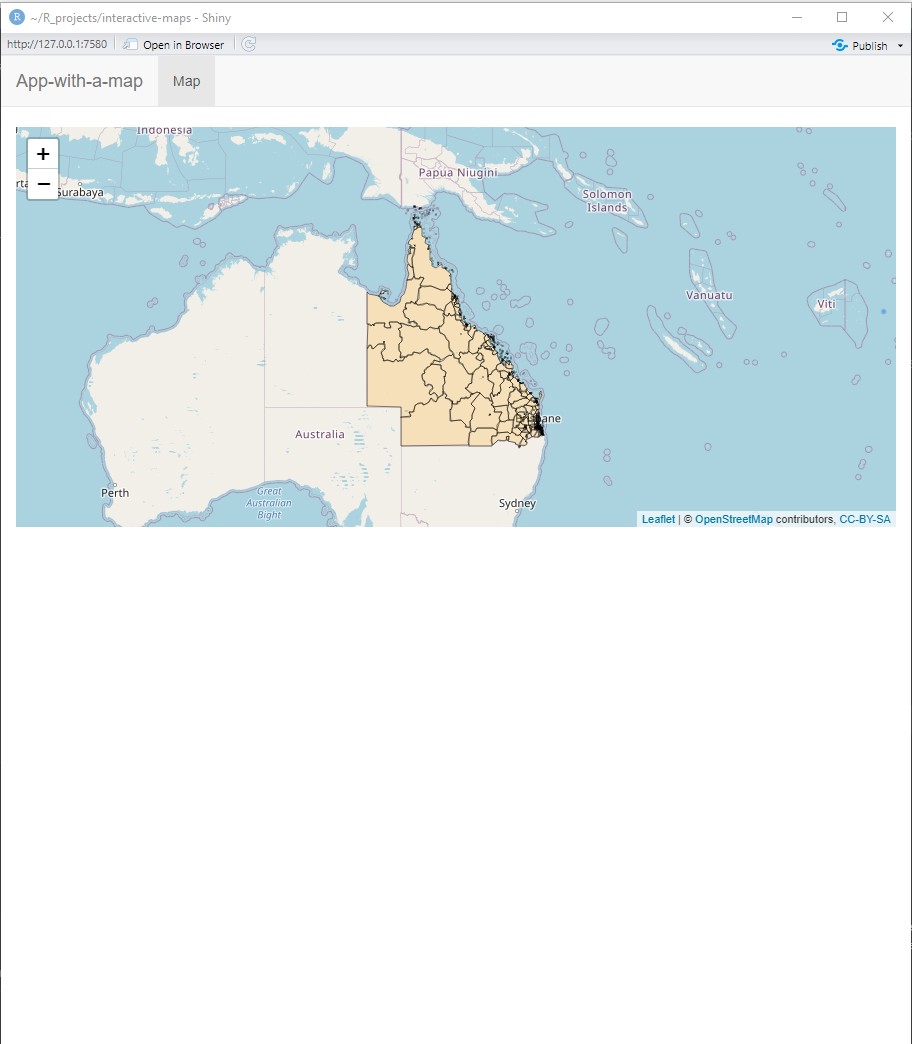
\includegraphics[width=3.125in,height=\textheight]{www/app-images/02-first-leaflet-map.png}

\begin{Shaded}
\begin{Highlighting}[]
\NormalTok{shiny}\SpecialCharTok{::}\FunctionTok{runGitHub}\NormalTok{(}\StringTok{"RWParsons/interactive{-}maps"}\NormalTok{, }\AttributeTok{subdir=}\StringTok{"input/apps/02{-}first{-}leaflet{-}map/"}\NormalTok{)}
\end{Highlighting}
\end{Shaded}

\hypertarget{filling-the-space}{%
\subsection{Filling the space}\label{filling-the-space}}

You might notice a few things here that you'd like to change with the ui already. Without getting into details like the colours of the panels, a major issue is that the map doesn't fill the entire space in the panel. Before we get into user-inputs, and for my own sanity, this has to be fixed.

Unfortunately, this is a surprisingly annoying thing to do. If you change the height and width of the map to be 100\% of the viewport height and width (by using \texttt{height="100vh",\ width="100vw"} in \texttt{leafletOutput()}) then you end up with a padding distance between the map and the panel, and an offset from above due to the height of the top panel bar. The best solution is to create a division (\texttt{div}), remove its padding, and fill the space left with the map (100\%). This means a little bit of CSS code and then assigning it to the division which wraps the map. I get the CSS code and the division to talk to eachother by assigning the class of the division to be `outer' and assigning the aesthetic changes to `div.outer' in the CSS code. The 41px that I remove at the top is due to the top bar of the navbarPage being 41px high.

\begin{Shaded}
\begin{Highlighting}[]
\FunctionTok{library}\NormalTok{(shiny)}
\FunctionTok{library}\NormalTok{(leaflet)}
\FunctionTok{library}\NormalTok{(tidyverse)}
\FunctionTok{library}\NormalTok{(sf)}
\NormalTok{input\_dir }\OtherTok{\textless{}{-}} \StringTok{"./input"}

\NormalTok{sa2\_polygons }\OtherTok{\textless{}{-}} \FunctionTok{readRDS}\NormalTok{(}\FunctionTok{file.path}\NormalTok{(input\_dir, }\StringTok{"stacked\_SA1\_and\_SA2\_polygons\_year2016\_simplified.rds"}\NormalTok{)) }\SpecialCharTok{\%\textgreater{}\%}
  \FunctionTok{filter}\NormalTok{(SA\_level}\SpecialCharTok{==}\DecValTok{2}\NormalTok{)}

\NormalTok{ui }\OtherTok{\textless{}{-}} \FunctionTok{navbarPage}\NormalTok{(}
  \StringTok{"App{-}with{-}a{-}map"}\NormalTok{, }\AttributeTok{id=}\StringTok{"nav"}\NormalTok{,}
  \FunctionTok{tabPanel}\NormalTok{(}
    \StringTok{"Map"}\NormalTok{,}
    \FunctionTok{div}\NormalTok{(}
      \AttributeTok{class=}\StringTok{"outer"}\NormalTok{,}
\NormalTok{        tags}\SpecialCharTok{$}\FunctionTok{head}\NormalTok{(}
\NormalTok{          tags}\SpecialCharTok{$}\FunctionTok{style}\NormalTok{(}\FunctionTok{HTML}\NormalTok{(}\StringTok{"}
\StringTok{            div.outer \{}
\StringTok{              position: fixed;}
\StringTok{              top: 41px;}
\StringTok{              left: 0;}
\StringTok{              right: 0;}
\StringTok{              bottom: 0;}
\StringTok{              overflow: hidden;}
\StringTok{              padding: 0;}
\StringTok{            \}}
\StringTok{            "}
\NormalTok{          ))}
\NormalTok{        ),}
      \FunctionTok{leafletOutput}\NormalTok{(}\StringTok{\textquotesingle{}map\textquotesingle{}}\NormalTok{, }\AttributeTok{height=}\StringTok{"100\%"}\NormalTok{, }\AttributeTok{width=}\StringTok{"100\%"}\NormalTok{)}
\NormalTok{    )}
\NormalTok{  )}
\NormalTok{)}

\NormalTok{server }\OtherTok{\textless{}{-}} \ControlFlowTok{function}\NormalTok{(input, output, session) \{}
\NormalTok{  output}\SpecialCharTok{$}\NormalTok{map }\OtherTok{\textless{}{-}} \FunctionTok{renderLeaflet}\NormalTok{(\{}
    \FunctionTok{leaflet}\NormalTok{() }\SpecialCharTok{\%\textgreater{}\%}
      \FunctionTok{addTiles}\NormalTok{() }\SpecialCharTok{\%\textgreater{}\%}
      \FunctionTok{addPolygons}\NormalTok{(}
        \AttributeTok{data=}\NormalTok{sa2\_polygons,}
        \AttributeTok{fillColor=}\StringTok{"Orange"}\NormalTok{,}
        \AttributeTok{color=}\StringTok{"black"}\NormalTok{,}
        \AttributeTok{weight=}\DecValTok{1}\NormalTok{,}
        \AttributeTok{group=}\StringTok{"Polygons"}
\NormalTok{      )}
\NormalTok{  \})}
\NormalTok{\}}

\FunctionTok{shinyApp}\NormalTok{(ui, server)}
\end{Highlighting}
\end{Shaded}

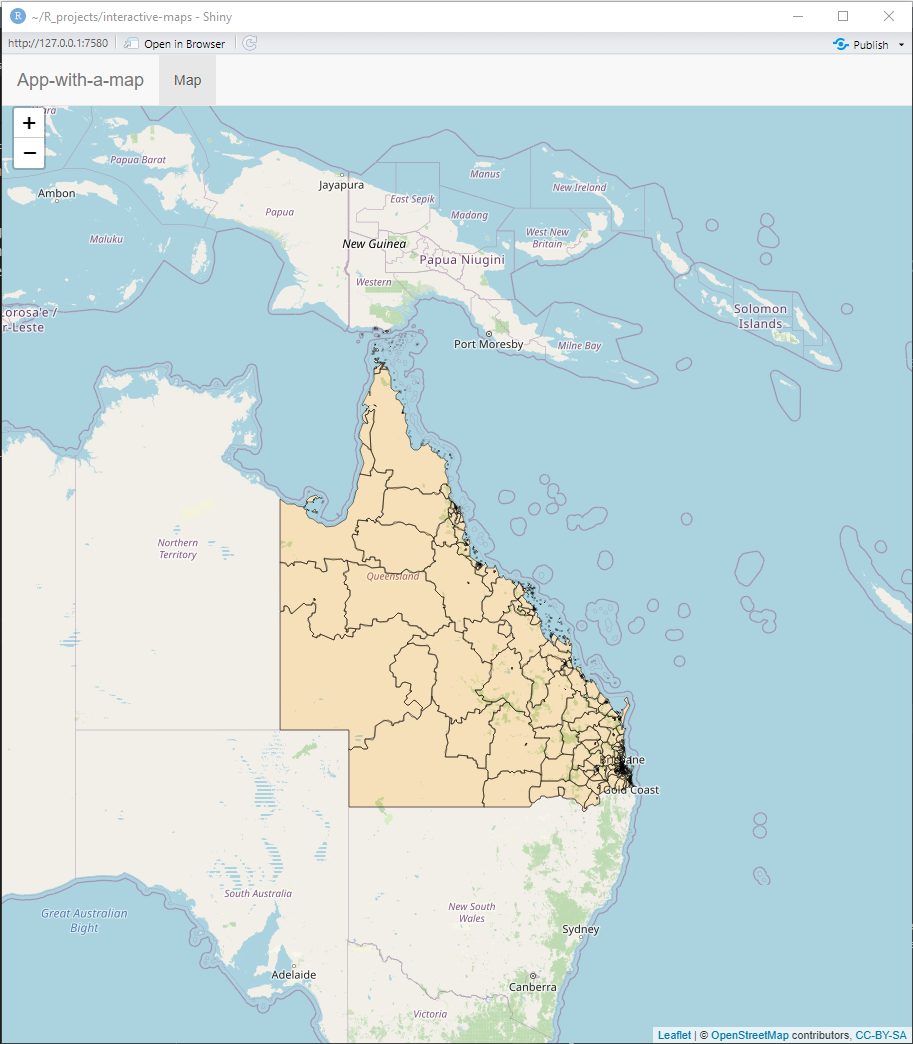
\includegraphics[width=3.125in,height=\textheight]{www/app-images/03-fill-panel-with-css.png}

\begin{Shaded}
\begin{Highlighting}[]
\NormalTok{shiny}\SpecialCharTok{::}\FunctionTok{runGitHub}\NormalTok{(}\StringTok{"RWParsons/interactive{-}maps"}\NormalTok{, }\AttributeTok{subdir=}\StringTok{"input/apps/03{-}fill{-}panel{-}with{-}css/"}\NormalTok{)}
\end{Highlighting}
\end{Shaded}

Now we have an app with a map, not just an app with a map (and painfully empty space).

\includegraphics[width=3.125in,height=\textheight]{www/phew.gif}

\hypertarget{leaflet-vs-shiny-interactivity}{%
\section{Leaflet vs shiny interactivity}\label{leaflet-vs-shiny-interactivity}}

There are interactive elements which come in leaflet before even incorporating shiny. For example, in the previous chapter we made a leaflet map that had a layer selector which gives the user control over what polygon layer (SA1, SA2, SA3) was being displayed on the map. This functionality is all leaflet based and incorporating it into a shiny app doesn't require adding any inputs to the ui side of the shiny app! This is great, because it doesn't depend on the server side to do any heavy lifting, and it can be functional while the server side is busy doing other operations. If possible, it's best to make use of this interactivity that leaflet has to offer: this means less code to maintain and less work for the server where you host your shiny app.

However, we will need to incorporate shiny inputs at the point where we want to add features to our app that leaflet doesn't have for us. To do this, we update our map very differently to how we updated the histogram in our first app example. Re-making the map is computationally expensive and would drastically slow down how quick the map responds to your inputs. In the histogram example, we used the following code.

\begin{Shaded}
\begin{Highlighting}[]
\NormalTok{output}\SpecialCharTok{$}\NormalTok{plot }\OtherTok{\textless{}{-}} \FunctionTok{renderPlot}\NormalTok{(}\AttributeTok{expr=}\NormalTok{\{}
  \FunctionTok{hist}\NormalTok{(}\AttributeTok{x=}\FunctionTok{rnorm}\NormalTok{(input}\SpecialCharTok{$}\NormalTok{n))}
\NormalTok{\})}
\end{Highlighting}
\end{Shaded}

\texttt{renderPlot()} takes a few arguments but the one we care most about is the first: \texttt{expr}. Since it's always the first argument of all the \texttt{render\_\_\_()} functions, we don't normally bother with the \texttt{expr=}. This is the expression (code) that creates the plot. Since it reads an input, every time that the \texttt{input\$n} is updated, the server side reacts by updating it's output which is then displayed to the user.

For our leaflet maps, we don't want to use user inputs in our \texttt{renderLeaflet()} expression as this would mean redrawing the content delays for the user. Instead, we observe changes to the inputs and update our map via a proxy.

In the app below, we add some leaflet interactivity as well as some shiny reactivity.

This map has a toggle to switch between showing the polygons and towns. Also, clicking on the markers for the towns will show a popup. The popup content is assigned when adding the circle markers (\texttt{addCircleMarkers()}) and you can use HTML tags to customise how it displays. All of this interactivity was made when we first rendered the leaflet map.

We also added an panel to hold a drop down menu containing names of all the towns that we have on the plot. If you select a town, this updates the input\(town_name which triggers some reactivity since it is being observed. When a town is selected, the map will zoom to its coordinates. If none is selected, it zooms out to look at all of Queensland. This part is controlled by shiny reactivity. It updates the existing map by using `leafletProxy()`. This takes one argument: the id of the map, which is the same as the output id (we used `output\)map\texttt{)\ so\ we\ update\ our\ map\ with}leafletProxy(mapId=``map'')\texttt{.\ This\ functionality\ is\ only\ for\ shiny\ apps\ and\ shiny\ docs,\ it\ allows\ us\ to\ add\ or\ modify\ content\ on\ our\ existing\ map\ without\ having\ to\ render\ it\ again.\ We\ used\ the}flyTo\texttt{and}flyToBounds` functions to update our map to move to the given location. However, we could can make all sorts of modifications and additions to our map in this way!

\begin{Shaded}
\begin{Highlighting}[]
\FunctionTok{library}\NormalTok{(shiny)}
\FunctionTok{library}\NormalTok{(leaflet)}
\FunctionTok{library}\NormalTok{(tidyverse)}
\FunctionTok{library}\NormalTok{(sf)}
\NormalTok{input\_dir }\OtherTok{\textless{}{-}} \StringTok{"./input"}

\NormalTok{sa2\_polygons }\OtherTok{\textless{}{-}} \FunctionTok{readRDS}\NormalTok{(}\FunctionTok{file.path}\NormalTok{(input\_dir, }\StringTok{"stacked\_SA1\_and\_SA2\_polygons\_year2016\_simplified.rds"}\NormalTok{)) }\SpecialCharTok{\%\textgreater{}\%}
  \FunctionTok{filter}\NormalTok{(SA\_level}\SpecialCharTok{==}\DecValTok{2}\NormalTok{)}

\NormalTok{towns }\OtherTok{\textless{}{-}} \FunctionTok{read.csv}\NormalTok{(}\FunctionTok{file.path}\NormalTok{(input\_dir, }\StringTok{"df\_towns.csv"}\NormalTok{)) }

\NormalTok{ui }\OtherTok{\textless{}{-}} \FunctionTok{navbarPage}\NormalTok{(}
  \StringTok{"App{-}with{-}a{-}map"}\NormalTok{, }\AttributeTok{id=}\StringTok{"nav"}\NormalTok{,}
  \FunctionTok{tabPanel}\NormalTok{(}
    \StringTok{"Map"}\NormalTok{,}
    \FunctionTok{div}\NormalTok{(}
      \AttributeTok{class=}\StringTok{"outer"}\NormalTok{,}
\NormalTok{        tags}\SpecialCharTok{$}\FunctionTok{head}\NormalTok{(}
\NormalTok{          tags}\SpecialCharTok{$}\FunctionTok{style}\NormalTok{(}\FunctionTok{HTML}\NormalTok{(}\StringTok{"}
\StringTok{            div.outer \{}
\StringTok{              position: fixed;}
\StringTok{              top: 41px;}
\StringTok{              left: 0;}
\StringTok{              right: 0;}
\StringTok{              bottom: 0;}
\StringTok{              overflow: hidden;}
\StringTok{              padding: 0;}
\StringTok{            \}}
\StringTok{            "}
\NormalTok{          ))}
\NormalTok{        ),}
      \FunctionTok{leafletOutput}\NormalTok{(}\StringTok{\textquotesingle{}map\textquotesingle{}}\NormalTok{, }\AttributeTok{height=}\StringTok{"100\%"}\NormalTok{, }\AttributeTok{width=}\StringTok{"100\%"}\NormalTok{),}
      \FunctionTok{absolutePanel}\NormalTok{(}
        \AttributeTok{top=}\DecValTok{75}\NormalTok{, }\AttributeTok{left=}\DecValTok{10}\NormalTok{, }
        \AttributeTok{class =} \StringTok{"panel panel{-}default"}\NormalTok{,}
        \FunctionTok{selectInput}\NormalTok{(}\StringTok{\textquotesingle{}town\_name\textquotesingle{}}\NormalTok{, }\StringTok{\textquotesingle{}Town Name\textquotesingle{}}\NormalTok{,}
                  \AttributeTok{choices =} \FunctionTok{c}\NormalTok{(}\StringTok{\textquotesingle{}None\textquotesingle{}}\NormalTok{, }\FunctionTok{sort}\NormalTok{(towns}\SpecialCharTok{$}\NormalTok{location)),}
                  \AttributeTok{selected =} \StringTok{"None"}\NormalTok{)}
\NormalTok{      )}
\NormalTok{    )}
\NormalTok{  )}
\NormalTok{)}

\NormalTok{server }\OtherTok{\textless{}{-}} \ControlFlowTok{function}\NormalTok{(input, output, session) \{}
  
  \FunctionTok{observe}\NormalTok{(\{}
    \ControlFlowTok{if}\NormalTok{(input}\SpecialCharTok{$}\NormalTok{town\_name}\SpecialCharTok{!=}\StringTok{"None"}\NormalTok{) \{}
\NormalTok{      town\_df }\OtherTok{\textless{}{-}}\NormalTok{ towns[towns}\SpecialCharTok{$}\NormalTok{location}\SpecialCharTok{==}\NormalTok{input}\SpecialCharTok{$}\NormalTok{town\_name, ]}
      \FunctionTok{leafletProxy}\NormalTok{(}\StringTok{"map"}\NormalTok{) }\SpecialCharTok{\%\textgreater{}\%}
        \FunctionTok{flyTo}\NormalTok{(}\AttributeTok{lng=}\NormalTok{town\_df}\SpecialCharTok{$}\NormalTok{x, }\AttributeTok{lat=}\NormalTok{town\_df}\SpecialCharTok{$}\NormalTok{y, }\AttributeTok{zoom=}\DecValTok{10}\NormalTok{)}
\NormalTok{    \} }\ControlFlowTok{else}\NormalTok{ \{}
      \FunctionTok{leafletProxy}\NormalTok{(}\StringTok{"map"}\NormalTok{) }\SpecialCharTok{\%\textgreater{}\%}
        \FunctionTok{flyToBounds}\NormalTok{(}
          \AttributeTok{lng1 =} \FloatTok{137.725724}\NormalTok{, }\AttributeTok{lat1 =} \SpecialCharTok{{-}}\FloatTok{28.903687}\NormalTok{, }
          \AttributeTok{lng2 =} \FloatTok{151.677076}\NormalTok{, }\AttributeTok{lat2 =} \SpecialCharTok{{-}}\FloatTok{10.772608}
\NormalTok{        )}
\NormalTok{    \}}
\NormalTok{  \})}
  
\NormalTok{  output}\SpecialCharTok{$}\NormalTok{map }\OtherTok{\textless{}{-}} \FunctionTok{renderLeaflet}\NormalTok{(\{}
    \FunctionTok{leaflet}\NormalTok{() }\SpecialCharTok{\%\textgreater{}\%}
      \FunctionTok{addTiles}\NormalTok{() }\SpecialCharTok{\%\textgreater{}\%}
      \FunctionTok{addPolygons}\NormalTok{(}
        \AttributeTok{data=}\NormalTok{sa2\_polygons,}
        \AttributeTok{fillColor=}\StringTok{"Orange"}\NormalTok{,}
        \AttributeTok{color=}\StringTok{"black"}\NormalTok{,}
        \AttributeTok{weight=}\DecValTok{1}\NormalTok{,}
        \AttributeTok{group=}\StringTok{"Polygons"}
\NormalTok{      ) }\SpecialCharTok{\%\textgreater{}\%}
      \FunctionTok{addCircleMarkers}\NormalTok{(}
        \AttributeTok{lng=}\NormalTok{towns}\SpecialCharTok{$}\NormalTok{x,}
        \AttributeTok{lat=}\NormalTok{towns}\SpecialCharTok{$}\NormalTok{y,}
        \AttributeTok{popup=}\NormalTok{glue}\SpecialCharTok{::}\FunctionTok{glue}\NormalTok{(}\StringTok{"\textless{}b\textgreater{}Location:\textless{}/b\textgreater{} \{towns$acute\_care\_centre\}"}\NormalTok{),}
        \AttributeTok{radius=}\DecValTok{2}\NormalTok{, }
        \AttributeTok{fillOpacity=}\DecValTok{0}\NormalTok{,}
        \AttributeTok{group=}\StringTok{"Towns"}
\NormalTok{      ) }\SpecialCharTok{\%\textgreater{}\%}
      \FunctionTok{addLayersControl}\NormalTok{(}
        \AttributeTok{position=}\StringTok{"topright"}\NormalTok{,}
        \AttributeTok{baseGroups=}\FunctionTok{c}\NormalTok{(}\StringTok{"None"}\NormalTok{, }\StringTok{"Polygons"}\NormalTok{),}
        \AttributeTok{overlayGroups=}\FunctionTok{c}\NormalTok{(}\StringTok{"Towns"}\NormalTok{),}
        \AttributeTok{options=}\FunctionTok{layersControlOptions}\NormalTok{(}\AttributeTok{collapsed =} \ConstantTok{FALSE}\NormalTok{)}
\NormalTok{      )}
\NormalTok{  \})}
\NormalTok{\}}

\FunctionTok{shinyApp}\NormalTok{(ui, server)}
\end{Highlighting}
\end{Shaded}

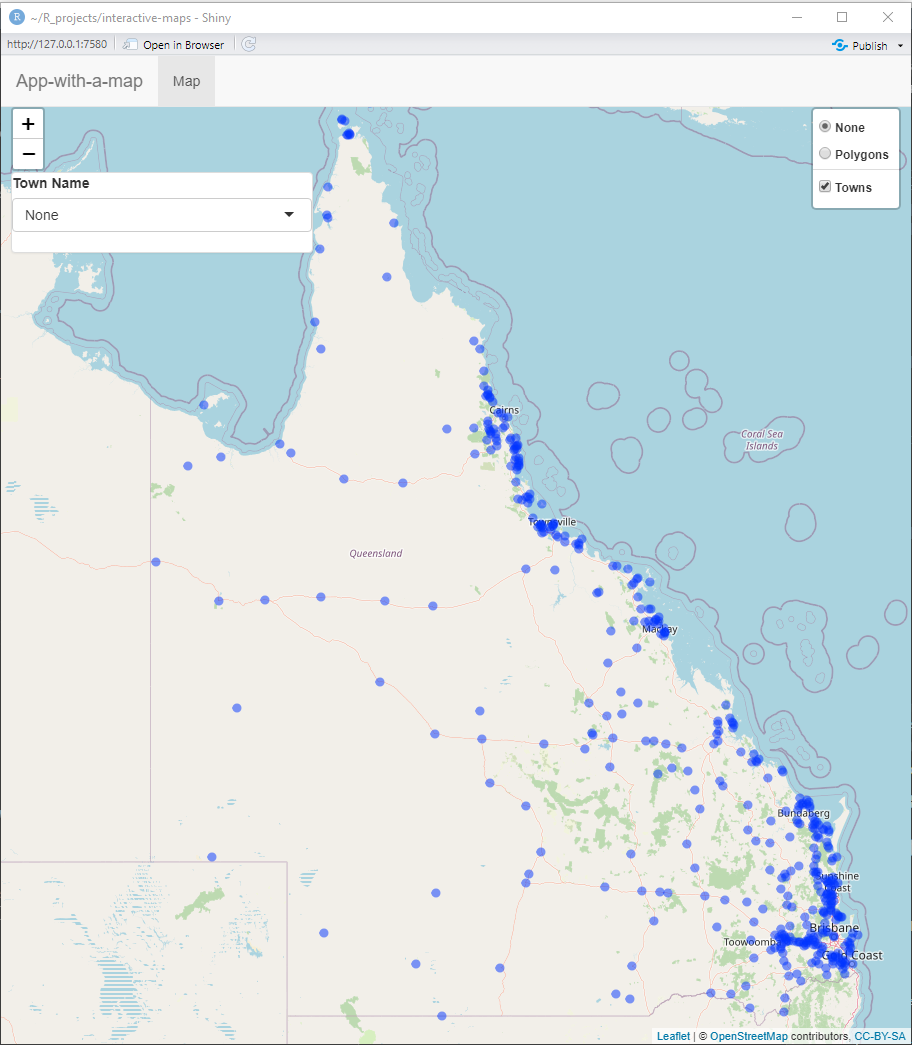
\includegraphics[width=3.125in,height=\textheight]{www/app-images/04-leaflet-and-shiny-interactivity.png}

\begin{Shaded}
\begin{Highlighting}[]
\NormalTok{shiny}\SpecialCharTok{::}\FunctionTok{runGitHub}\NormalTok{(}\StringTok{"RWParsons/interactive{-}maps"}\NormalTok{, }\AttributeTok{subdir=}\StringTok{"input/apps/04{-}leaflet{-}and{-}shiny{-}interactivity/"}\NormalTok{)}
\end{Highlighting}
\end{Shaded}

We used a range of features from both leaflet and shiny to make iTRAQI interactive. This was a very brief introduction to reactivity and shiny. I recommend reading the \href{https://mastering-shiny.org/basic-app.html}{sections 1-3 of Mastering Shiny} as the next chapter will cover specific tricks to add specific features to your maps won't do as good of a job introducing the fundamentals of shiny as Mastering Shiny does.

\hypertarget{iTRAQI-tricks}{%
\chapter{iTRAQI tricks}\label{iTRAQI-tricks}}

This is the beginning of the second part of the book, where all the iTRAQI tricks are detailed.

\begin{itemize}
\tightlist
\item
  Chapter \ref{async-loading}: Asynchronous loading and distracting your user
\item
  Mixing continuous and discrete colour palettes
\item
  Layer selection from the control panel

  \begin{itemize}
  \tightlist
  \item
    \texttt{addLayersControl} vs controls in shiny
  \item
    Updating the map
  \item
    Updating the legend
  \end{itemize}
\item
  Polygon filters

  \begin{itemize}
  \tightlist
  \item
    Filters from checkboxes
  \item
    Adding all/none to checkboxes
  \end{itemize}
\item
  Updating polygon aesthetics

  \begin{itemize}
  \tightlist
  \item
    \texttt{layerId} vs \texttt{group}
  \item
    Adding javascript to leaflet
  \item
    Updating fillColor and labels
  \end{itemize}
\item
  Showing a plot in parallel to your map

  \begin{itemize}
  \tightlist
  \item
    Matching your colour palette between the map and plot
  \item
    Interact with your map from the plot
  \end{itemize}
\item
  Getting predictions on \texttt{map\_click()}
\item
  Tours

  \begin{itemize}
  \tightlist
  \item
    Associating tour progression to map content
  \item
    Delayed content
  \end{itemize}
\item
  Information page
\end{itemize}

\hypertarget{async-loading}{%
\chapter{iTRAQI tricks}\label{async-loading}}

\hypertarget{asynchronous-loading-distracting-your-user}{%
\section{Asynchronous loading distracting your user}\label{asynchronous-loading-distracting-your-user}}

We made the following app in the last section of chapter \ref{shiny-intro} except we only used SA2 polygons. In the iTRAQI app, we use both SA1s and SA2s - this means a lot more detail, many more polygons, and a slower load time. The following code loads both SA1s and SA2s - note how long it takes to run by either copy-pasting the code or running the first \texttt{runGithub} line. (Also, appreciate that a shiny server may load it even slower than the computer, especially if that server has many concurrent users!)

\begin{Shaded}
\begin{Highlighting}[]
\NormalTok{shiny}\SpecialCharTok{::}\FunctionTok{runGitHub}\NormalTok{(}\StringTok{"RWParsons/interactive{-}maps"}\NormalTok{, }\AttributeTok{subdir=}\StringTok{"input/apps/05{-}async{-}load{-}1/"}\NormalTok{)}
\end{Highlighting}
\end{Shaded}

\begin{Shaded}
\begin{Highlighting}[]
\FunctionTok{library}\NormalTok{(shiny)}
\FunctionTok{library}\NormalTok{(leaflet)}
\FunctionTok{library}\NormalTok{(tidyverse)}
\FunctionTok{library}\NormalTok{(sf)}
\NormalTok{input\_dir }\OtherTok{\textless{}{-}} \StringTok{"./input"}

\NormalTok{sa\_polygons }\OtherTok{\textless{}{-}} \FunctionTok{readRDS}\NormalTok{(}\FunctionTok{file.path}\NormalTok{(input\_dir, }\StringTok{"stacked\_SA1\_and\_SA2\_polygons\_year2016\_simplified.rds"}\NormalTok{))}

\NormalTok{towns }\OtherTok{\textless{}{-}} \FunctionTok{read.csv}\NormalTok{(}\FunctionTok{file.path}\NormalTok{(input\_dir, }\StringTok{"df\_towns.csv"}\NormalTok{)) }

\NormalTok{ui }\OtherTok{\textless{}{-}} \FunctionTok{navbarPage}\NormalTok{(}
  \StringTok{"App{-}with{-}a{-}map"}\NormalTok{, }\AttributeTok{id=}\StringTok{"nav"}\NormalTok{,}
  \FunctionTok{tabPanel}\NormalTok{(}
    \StringTok{"Map"}\NormalTok{,}
    \FunctionTok{div}\NormalTok{(}
      \AttributeTok{class=}\StringTok{"outer"}\NormalTok{,}
\NormalTok{        tags}\SpecialCharTok{$}\FunctionTok{head}\NormalTok{(}
\NormalTok{          tags}\SpecialCharTok{$}\FunctionTok{style}\NormalTok{(}\FunctionTok{HTML}\NormalTok{(}\StringTok{"}
\StringTok{            div.outer \{}
\StringTok{              position: fixed;}
\StringTok{              top: 41px;}
\StringTok{              left: 0;}
\StringTok{              right: 0;}
\StringTok{              bottom: 0;}
\StringTok{              overflow: hidden;}
\StringTok{              padding: 0;}
\StringTok{            \}}
\StringTok{            "}
\NormalTok{          ))}
\NormalTok{        ),}
      \FunctionTok{leafletOutput}\NormalTok{(}\StringTok{\textquotesingle{}map\textquotesingle{}}\NormalTok{, }\AttributeTok{height=}\StringTok{"100\%"}\NormalTok{, }\AttributeTok{width=}\StringTok{"100\%"}\NormalTok{)}
\NormalTok{    )}
\NormalTok{  )}
\NormalTok{)}

\NormalTok{server }\OtherTok{\textless{}{-}} \ControlFlowTok{function}\NormalTok{(input, output, session) \{}
\NormalTok{  output}\SpecialCharTok{$}\NormalTok{map }\OtherTok{\textless{}{-}} \FunctionTok{renderLeaflet}\NormalTok{(\{}
    \FunctionTok{leaflet}\NormalTok{() }\SpecialCharTok{\%\textgreater{}\%}
      \FunctionTok{addTiles}\NormalTok{() }\SpecialCharTok{\%\textgreater{}\%}
      \FunctionTok{addPolygons}\NormalTok{(}
        \AttributeTok{data=}\NormalTok{sa\_polygons,}
        \AttributeTok{fillColor=}\StringTok{"Orange"}\NormalTok{,}
        \AttributeTok{color=}\StringTok{"black"}\NormalTok{,}
        \AttributeTok{weight=}\DecValTok{1}\NormalTok{,}
        \AttributeTok{group=}\StringTok{"Polygons"}
\NormalTok{      ) }\SpecialCharTok{\%\textgreater{}\%}
      \FunctionTok{addCircleMarkers}\NormalTok{(}
        \AttributeTok{lng=}\NormalTok{towns}\SpecialCharTok{$}\NormalTok{x,}
        \AttributeTok{lat=}\NormalTok{towns}\SpecialCharTok{$}\NormalTok{y,}
        \AttributeTok{popup=}\NormalTok{glue}\SpecialCharTok{::}\FunctionTok{glue}\NormalTok{(}\StringTok{"\textless{}b\textgreater{}Location:\textless{}/b\textgreater{} \{towns$acute\_care\_centre\}"}\NormalTok{),}
        \AttributeTok{radius=}\DecValTok{2}\NormalTok{, }
        \AttributeTok{fillOpacity=}\DecValTok{0}\NormalTok{,}
        \AttributeTok{group=}\StringTok{"Towns"}
\NormalTok{      ) }\SpecialCharTok{\%\textgreater{}\%}
      \FunctionTok{addLayersControl}\NormalTok{(}
        \AttributeTok{position=}\StringTok{"topright"}\NormalTok{,}
        \AttributeTok{baseGroups=}\FunctionTok{c}\NormalTok{(}\StringTok{"None"}\NormalTok{, }\StringTok{"Polygons"}\NormalTok{),}
        \AttributeTok{overlayGroups=}\FunctionTok{c}\NormalTok{(}\StringTok{"Towns"}\NormalTok{),}
        \AttributeTok{options=}\FunctionTok{layersControlOptions}\NormalTok{(}\AttributeTok{collapsed =} \ConstantTok{FALSE}\NormalTok{)}
\NormalTok{      )}
\NormalTok{  \})}
\NormalTok{\}}

\FunctionTok{shinyApp}\NormalTok{(ui, server)}
\end{Highlighting}
\end{Shaded}

There are a couple things that we can do to ensure our user doesn't get bored and close the app.
The first (and easiest) is to show a fun fact, loading spinner or some other form of brief entertainment. The second option is to load the map asynchronously: we can load part of the map and allow the user access to some of the functionality, and defer loading the computationally expensive parts a bit. For the iTRAQI app, we use both a fun fact/gif/image and asynchronous loading.

To show content, we will add a panel which displays over the app, and once the map is created, we will hide it.

To do this, we add an \texttt{absolutePanel()} to our UI which has the message and image that we want to display. Here, I use a function, \texttt{get\_display()} which gets a random message from those in \texttt{loading\_panel\_displays}. I format the messages using HTML and therefore need to wrap the display with \texttt{HTML()} when presenting it in the\texttt{absolutePanel}. Images can be added - here I have used some online but if you have images in the \texttt{www/} directory of your shiny app, you can use those instead.
To hide the panel once the map is created, we need to use \texttt{\{shinyjs\}}. To allow us to use it's functions on the UI, we need to include \texttt{useShinyjs()} there. Once the map is made in \texttt{renderLeafet()} on the server side, I hide the absolute panel with \texttt{shinyjs::hide("loadingScreen")}.

\begin{Shaded}
\begin{Highlighting}[]
\FunctionTok{library}\NormalTok{(shiny)}
\FunctionTok{library}\NormalTok{(leaflet)}
\FunctionTok{library}\NormalTok{(tidyverse)}
\FunctionTok{library}\NormalTok{(sf)}
\FunctionTok{library}\NormalTok{(glue)}
\FunctionTok{library}\NormalTok{(shinyjs)}

\NormalTok{input\_dir }\OtherTok{\textless{}{-}} \StringTok{"./input"}

\NormalTok{sa\_polygons }\OtherTok{\textless{}{-}} \FunctionTok{readRDS}\NormalTok{(}\FunctionTok{file.path}\NormalTok{(input\_dir, }\StringTok{"stacked\_SA1\_and\_SA2\_polygons\_year2016\_simplified.rds"}\NormalTok{))}
\NormalTok{towns }\OtherTok{\textless{}{-}} \FunctionTok{read.csv}\NormalTok{(}\FunctionTok{file.path}\NormalTok{(input\_dir, }\StringTok{"df\_towns.csv"}\NormalTok{)) }

\NormalTok{loading\_panel\_displays }\OtherTok{\textless{}{-}} \FunctionTok{c}\NormalTok{(}
  \FunctionTok{paste}\NormalTok{(}
    \AttributeTok{sep=}\StringTok{"\textless{}br\textgreater{}"}\NormalTok{,}
    \StringTok{"\textless{}h2\textgreater{}First fun fact text!\textless{}/h2\textgreater{}"}\NormalTok{,}
    \StringTok{\textquotesingle{}\textless{}img src="https://www.r{-}project.org/logo/Rlogo.png" alt="R" style="width:200px"\textgreater{}\textquotesingle{}}
\NormalTok{  ),}
  \FunctionTok{paste}\NormalTok{(}
    \AttributeTok{sep=}\StringTok{"\textless{}br\textgreater{}"}\NormalTok{,}
    \StringTok{"\textless{}h2\textgreater{}Second fun fact text!\textless{}/h2\textgreater{}"}\NormalTok{,}
    \StringTok{\textquotesingle{}\textless{}img src="https://www.rstudio.com/assets/img/logo.svg" alt="dog{-}1" style="width:200px;"\textgreater{}\textquotesingle{}}
\NormalTok{  )}
\NormalTok{)}

\NormalTok{get\_display }\OtherTok{\textless{}{-}} \ControlFlowTok{function}\NormalTok{() \{}
\NormalTok{  loading\_panel\_displays[}\FunctionTok{sample}\NormalTok{(}\DecValTok{1}\SpecialCharTok{:}\FunctionTok{length}\NormalTok{(loading\_panel\_displays), }\AttributeTok{size=}\DecValTok{1}\NormalTok{)]}
\NormalTok{\}}

\NormalTok{ui }\OtherTok{\textless{}{-}} \FunctionTok{navbarPage}\NormalTok{(}
  \StringTok{"App{-}with{-}a{-}map"}\NormalTok{, }\AttributeTok{id=}\StringTok{"nav"}\NormalTok{,}
  \FunctionTok{tabPanel}\NormalTok{(}
    \StringTok{"Map"}\NormalTok{,}
    \FunctionTok{useShinyjs}\NormalTok{(),}
    \FunctionTok{div}\NormalTok{(}
      \AttributeTok{class=}\StringTok{"outer"}\NormalTok{,}
\NormalTok{        tags}\SpecialCharTok{$}\FunctionTok{head}\NormalTok{(}
\NormalTok{          tags}\SpecialCharTok{$}\FunctionTok{style}\NormalTok{(}\FunctionTok{HTML}\NormalTok{(}\StringTok{"}
\StringTok{            div.outer \{}
\StringTok{              position: fixed;}
\StringTok{              top: 41px;}
\StringTok{              left: 0;}
\StringTok{              right: 0;}
\StringTok{              bottom: 0;}
\StringTok{              overflow: hidden;}
\StringTok{              padding: 0;}
\StringTok{            \}}
\StringTok{            "}
\NormalTok{          ))}
\NormalTok{        ),}
      \FunctionTok{leafletOutput}\NormalTok{(}\StringTok{\textquotesingle{}map\textquotesingle{}}\NormalTok{, }\AttributeTok{height=}\StringTok{"100\%"}\NormalTok{, }\AttributeTok{width=}\StringTok{"100\%"}\NormalTok{),}
      \FunctionTok{absolutePanel}\NormalTok{(}
        \AttributeTok{id =} \StringTok{"loadingScreen"}\NormalTok{, }\AttributeTok{class =} \StringTok{"panel panel{-}default"}\NormalTok{, }
        \AttributeTok{fixed =} \ConstantTok{TRUE}\NormalTok{, }\AttributeTok{draggable =} \ConstantTok{TRUE}\NormalTok{, }
        \AttributeTok{left =} \StringTok{"50\%"}\NormalTok{, }\AttributeTok{right =} \StringTok{"50\%"}\NormalTok{, }\AttributeTok{bottom =} \StringTok{"50\%"}\NormalTok{, }\AttributeTok{top=}\StringTok{"50\%"}\NormalTok{,}
        \AttributeTok{width =} \DecValTok{500}\NormalTok{, }\AttributeTok{height =} \DecValTok{200}\NormalTok{,}
        \FunctionTok{HTML}\NormalTok{(}\FunctionTok{get\_display}\NormalTok{())}
\NormalTok{      )}
\NormalTok{    )}
\NormalTok{  )}
\NormalTok{)}

\NormalTok{server }\OtherTok{\textless{}{-}} \ControlFlowTok{function}\NormalTok{(input, output, session) \{}
\NormalTok{  output}\SpecialCharTok{$}\NormalTok{map }\OtherTok{\textless{}{-}} \FunctionTok{renderLeaflet}\NormalTok{(\{}
\NormalTok{    map }\OtherTok{\textless{}{-}} \FunctionTok{leaflet}\NormalTok{() }\SpecialCharTok{\%\textgreater{}\%}
      \FunctionTok{addTiles}\NormalTok{() }\SpecialCharTok{\%\textgreater{}\%}
      \FunctionTok{addPolygons}\NormalTok{(}
        \AttributeTok{data=}\NormalTok{sa\_polygons,}
        \AttributeTok{fillColor=}\StringTok{"Orange"}\NormalTok{,}
        \AttributeTok{color=}\StringTok{"black"}\NormalTok{,}
        \AttributeTok{weight=}\DecValTok{1}\NormalTok{,}
        \AttributeTok{group=}\StringTok{"Polygons"}
\NormalTok{      ) }\SpecialCharTok{\%\textgreater{}\%}
      \FunctionTok{addCircleMarkers}\NormalTok{(}
        \AttributeTok{lng=}\NormalTok{towns}\SpecialCharTok{$}\NormalTok{x,}
        \AttributeTok{lat=}\NormalTok{towns}\SpecialCharTok{$}\NormalTok{y,}
        \AttributeTok{popup=}\NormalTok{glue}\SpecialCharTok{::}\FunctionTok{glue}\NormalTok{(}\StringTok{"\textless{}b\textgreater{}Location:\textless{}/b\textgreater{} \{towns$acute\_care\_centre\}"}\NormalTok{),}
        \AttributeTok{radius=}\DecValTok{2}\NormalTok{, }
        \AttributeTok{fillOpacity=}\DecValTok{0}\NormalTok{,}
        \AttributeTok{group=}\StringTok{"Towns"}
\NormalTok{      ) }\SpecialCharTok{\%\textgreater{}\%}
      \FunctionTok{addLayersControl}\NormalTok{(}
        \AttributeTok{position=}\StringTok{"topright"}\NormalTok{,}
        \AttributeTok{baseGroups=}\FunctionTok{c}\NormalTok{(}\StringTok{"None"}\NormalTok{, }\StringTok{"Polygons"}\NormalTok{),}
        \AttributeTok{overlayGroups=}\FunctionTok{c}\NormalTok{(}\StringTok{"Towns"}\NormalTok{),}
        \AttributeTok{options=}\FunctionTok{layersControlOptions}\NormalTok{(}\AttributeTok{collapsed =} \ConstantTok{FALSE}\NormalTok{)}
\NormalTok{      )}
    \FunctionTok{hide}\NormalTok{(}\StringTok{"loadingScreen"}\NormalTok{)}
\NormalTok{    map}
\NormalTok{  \})}
\NormalTok{\}}

\FunctionTok{shinyApp}\NormalTok{(ui, server)}
\end{Highlighting}
\end{Shaded}

\begin{Shaded}
\begin{Highlighting}[]
\NormalTok{shiny}\SpecialCharTok{::}\FunctionTok{runGitHub}\NormalTok{(}\StringTok{"RWParsons/interactive{-}maps"}\NormalTok{, }\AttributeTok{subdir=}\StringTok{"input/apps/06{-}async{-}load{-}2/"}\NormalTok{)}
\end{Highlighting}
\end{Shaded}

You might notice that there is still a delay between the loading screen disappearing and the map appearing. This is because there is still some time between when the map is rendered by the server and it being drawn for us to see.

Fortunately, we can make it easier to draw the initial map if it (initially) lacks the detailed polygons.

To load the map asynchronously, we will first render a relatively simple map - just the base tiles and the towns. Then, once that's displaying to the user, we will add the polygons with \texttt{leafletProxy()}.

To trigger this action, we will use a callback. \texttt{onFlushed()} can be used to register functions which occur after Shiny flushes the reactive system. In our case, we can use this to trigger the adding of polygons to our map once the first, simple map is ``flushed''.

Since in the iTRAQI app, we have more than one map, we trigger a function onFlushed that can trigger all maps, and only those maps on the current tab are triggered to add content asynchronously. Since we need to check whether (1) we have triggered ``to\_load'' the map, (2) whether the ``map'' exists to add content to, and (3) whether the map is already completed or not (``map\_complete''), we store these in reactive values. These are values which can be used to trigger events by observing them, and be updated within the server side. Every time content is flushed, the ``to\_load'' is updated, this triggers an observe event to add content to the map. If this finds that the map doesn't exist or it does and the additional content has already been added, it does nothing. If the map exists and it hasn't had the polygons added (\texttt{!is.null(rvs\$map)\ \&\ map\_complete==FALSE}), it adds them, and then updates the map\_complete to be TRUE (so that it won't add the polygons again).

The end result is that the initial map appears quickly and is interactive and the addition of the polygons happens in the background (hopefully before we try to display them). In this example, we hide the loading screen once we have added the polygons but if we are confident that the user is unlikely to try to show them within the first little bit since opening the app, we could move the \texttt{hide("loadingScreen")} back to the \texttt{renderLeafet()}.

\begin{Shaded}
\begin{Highlighting}[]
\FunctionTok{library}\NormalTok{(shiny)}
\FunctionTok{library}\NormalTok{(leaflet)}
\FunctionTok{library}\NormalTok{(tidyverse)}
\FunctionTok{library}\NormalTok{(sf)}
\FunctionTok{library}\NormalTok{(glue)}
\FunctionTok{library}\NormalTok{(shinyjs)}

\NormalTok{input\_dir }\OtherTok{\textless{}{-}} \StringTok{"./input"}

\NormalTok{sa\_polygons }\OtherTok{\textless{}{-}} \FunctionTok{readRDS}\NormalTok{(}\FunctionTok{file.path}\NormalTok{(input\_dir, }\StringTok{"stacked\_SA1\_and\_SA2\_polygons\_year2016\_simplified.rds"}\NormalTok{))}
\NormalTok{towns }\OtherTok{\textless{}{-}} \FunctionTok{read.csv}\NormalTok{(}\FunctionTok{file.path}\NormalTok{(input\_dir, }\StringTok{"df\_towns.csv"}\NormalTok{)) }

\NormalTok{loading\_panel\_displays }\OtherTok{\textless{}{-}} \FunctionTok{c}\NormalTok{(}
  \FunctionTok{paste}\NormalTok{(}
    \AttributeTok{sep=}\StringTok{"\textless{}br\textgreater{}"}\NormalTok{,}
    \StringTok{"\textless{}h2\textgreater{}First fun fact text!\textless{}/h2\textgreater{}"}\NormalTok{,}
    \StringTok{\textquotesingle{}\textless{}img src="https://www.r{-}project.org/logo/Rlogo.png" alt="R" style="width:200px"\textgreater{}\textquotesingle{}}
\NormalTok{  ),}
  \FunctionTok{paste}\NormalTok{(}
    \AttributeTok{sep=}\StringTok{"\textless{}br\textgreater{}"}\NormalTok{,}
    \StringTok{"\textless{}h2\textgreater{}Second fun fact text!\textless{}/h2\textgreater{}"}\NormalTok{,}
    \StringTok{\textquotesingle{}\textless{}img src="https://www.rstudio.com/assets/img/logo.svg" alt="dog{-}1" style="width:200px;"\textgreater{}\textquotesingle{}}
\NormalTok{  )}
\NormalTok{)}

\NormalTok{get\_display }\OtherTok{\textless{}{-}} \ControlFlowTok{function}\NormalTok{() \{}
\NormalTok{  loading\_panel\_displays[}\FunctionTok{sample}\NormalTok{(}\DecValTok{1}\SpecialCharTok{:}\FunctionTok{length}\NormalTok{(loading\_panel\_displays), }\AttributeTok{size=}\DecValTok{1}\NormalTok{)]}
\NormalTok{\}}

\NormalTok{ui }\OtherTok{\textless{}{-}} \FunctionTok{navbarPage}\NormalTok{(}
  \StringTok{"App{-}with{-}a{-}map"}\NormalTok{, }\AttributeTok{id=}\StringTok{"nav"}\NormalTok{,}
  \FunctionTok{tabPanel}\NormalTok{(}
    \StringTok{"Map"}\NormalTok{,}
    \FunctionTok{useShinyjs}\NormalTok{(),}
    \FunctionTok{div}\NormalTok{(}
      \AttributeTok{class=}\StringTok{"outer"}\NormalTok{,}
\NormalTok{        tags}\SpecialCharTok{$}\FunctionTok{head}\NormalTok{(}
\NormalTok{          tags}\SpecialCharTok{$}\FunctionTok{style}\NormalTok{(}\FunctionTok{HTML}\NormalTok{(}\StringTok{"}
\StringTok{            div.outer \{}
\StringTok{              position: fixed;}
\StringTok{              top: 41px;}
\StringTok{              left: 0;}
\StringTok{              right: 0;}
\StringTok{              bottom: 0;}
\StringTok{              overflow: hidden;}
\StringTok{              padding: 0;}
\StringTok{            \}}
\StringTok{            "}
\NormalTok{          ))}
\NormalTok{        ),}
      \FunctionTok{leafletOutput}\NormalTok{(}\StringTok{\textquotesingle{}map\textquotesingle{}}\NormalTok{, }\AttributeTok{height=}\StringTok{"100\%"}\NormalTok{, }\AttributeTok{width=}\StringTok{"100\%"}\NormalTok{),}
      \FunctionTok{absolutePanel}\NormalTok{(}
        \AttributeTok{top=}\DecValTok{75}\NormalTok{, }\AttributeTok{left=}\DecValTok{10}\NormalTok{, }
        \AttributeTok{class =} \StringTok{"panel panel{-}default"}\NormalTok{,}
        \FunctionTok{selectInput}\NormalTok{(}\StringTok{\textquotesingle{}town\_name\textquotesingle{}}\NormalTok{, }\StringTok{\textquotesingle{}Town Name\textquotesingle{}}\NormalTok{,}
                  \AttributeTok{choices =} \FunctionTok{c}\NormalTok{(}\StringTok{\textquotesingle{}None\textquotesingle{}}\NormalTok{, }\FunctionTok{sort}\NormalTok{(towns}\SpecialCharTok{$}\NormalTok{location)),}
                  \AttributeTok{selected =} \StringTok{"None"}\NormalTok{)}
\NormalTok{      ),}
      \FunctionTok{absolutePanel}\NormalTok{(}
        \AttributeTok{id =} \StringTok{"loadingScreen"}\NormalTok{, }\AttributeTok{class =} \StringTok{"panel panel{-}default"}\NormalTok{, }
        \AttributeTok{fixed =} \ConstantTok{TRUE}\NormalTok{, }\AttributeTok{draggable =} \ConstantTok{TRUE}\NormalTok{, }
        \AttributeTok{left =} \StringTok{"50\%"}\NormalTok{, }\AttributeTok{right =} \StringTok{"50\%"}\NormalTok{, }\AttributeTok{bottom =} \StringTok{"50\%"}\NormalTok{, }\AttributeTok{top=}\StringTok{"50\%"}\NormalTok{,}
        \AttributeTok{width =} \DecValTok{500}\NormalTok{, }\AttributeTok{height =} \DecValTok{200}\NormalTok{,}
        \FunctionTok{HTML}\NormalTok{(}\FunctionTok{get\_display}\NormalTok{())}
\NormalTok{      )}
\NormalTok{    )}
\NormalTok{  )}
\NormalTok{)}

\NormalTok{server }\OtherTok{\textless{}{-}} \ControlFlowTok{function}\NormalTok{(input, output, session) \{}
  
\NormalTok{  rvs }\OtherTok{\textless{}{-}} \FunctionTok{reactiveValues}\NormalTok{(}\AttributeTok{to\_load=}\ConstantTok{NULL}\NormalTok{, }\AttributeTok{map=}\ConstantTok{NULL}\NormalTok{, }\AttributeTok{map\_complete=}\ConstantTok{FALSE}\NormalTok{)}
  
\NormalTok{  f }\OtherTok{\textless{}{-}} \ControlFlowTok{function}\NormalTok{() \{}
    \ControlFlowTok{if}\NormalTok{(}\FunctionTok{is.null}\NormalTok{(}\FunctionTok{isolate}\NormalTok{(rvs}\SpecialCharTok{$}\NormalTok{to\_load))) rvs}\SpecialCharTok{$}\NormalTok{to\_load }\OtherTok{\textless{}{-}} \DecValTok{1}
    \ControlFlowTok{if}\NormalTok{(}\SpecialCharTok{!}\FunctionTok{is.null}\NormalTok{(}\FunctionTok{isolate}\NormalTok{(rvs}\SpecialCharTok{$}\NormalTok{to\_load)) }\SpecialCharTok{\&} 
       \SpecialCharTok{!}\FunctionTok{isolate}\NormalTok{(rvs}\SpecialCharTok{$}\NormalTok{map\_complete) }\SpecialCharTok{\&} 
       \SpecialCharTok{!}\FunctionTok{is.null}\NormalTok{(}\FunctionTok{isolate}\NormalTok{(rvs}\SpecialCharTok{$}\NormalTok{map)))\{}
\NormalTok{      rvs}\SpecialCharTok{$}\NormalTok{to\_load }\OtherTok{\textless{}{-}} \FunctionTok{isolate}\NormalTok{(rvs}\SpecialCharTok{$}\NormalTok{to\_load) }\SpecialCharTok{+} \DecValTok{1}
\NormalTok{    \}}
\NormalTok{  \}}
  
\NormalTok{  session}\SpecialCharTok{$}\FunctionTok{onFlushed}\NormalTok{(f, }\AttributeTok{once=}\ConstantTok{FALSE}\NormalTok{)}
  
\NormalTok{  output}\SpecialCharTok{$}\NormalTok{map }\OtherTok{\textless{}{-}} \FunctionTok{renderLeaflet}\NormalTok{(\{}
\NormalTok{    rvs}\SpecialCharTok{$}\NormalTok{map }\OtherTok{\textless{}{-}} 
      \FunctionTok{leaflet}\NormalTok{() }\SpecialCharTok{\%\textgreater{}\%}
      \FunctionTok{addTiles}\NormalTok{() }\SpecialCharTok{\%\textgreater{}\%}
      \FunctionTok{addCircleMarkers}\NormalTok{(}
        \AttributeTok{lng=}\NormalTok{towns}\SpecialCharTok{$}\NormalTok{x,}
        \AttributeTok{lat=}\NormalTok{towns}\SpecialCharTok{$}\NormalTok{y,}
        \AttributeTok{popup=}\NormalTok{glue}\SpecialCharTok{::}\FunctionTok{glue}\NormalTok{(}\StringTok{"\textless{}b\textgreater{}Location:\textless{}/b\textgreater{} \{towns$acute\_care\_centre\}"}\NormalTok{),}
        \AttributeTok{radius=}\DecValTok{2}\NormalTok{, }
        \AttributeTok{fillOpacity=}\DecValTok{0}\NormalTok{,}
        \AttributeTok{group=}\StringTok{"Towns"}
\NormalTok{      ) }\SpecialCharTok{\%\textgreater{}\%}
      \FunctionTok{addLayersControl}\NormalTok{(}
        \AttributeTok{position=}\StringTok{"topright"}\NormalTok{,}
        \AttributeTok{baseGroups=}\FunctionTok{c}\NormalTok{(}\StringTok{"None"}\NormalTok{, }\StringTok{"Polygons"}\NormalTok{),}
        \AttributeTok{overlayGroups=}\FunctionTok{c}\NormalTok{(}\StringTok{"Towns"}\NormalTok{),}
        \AttributeTok{options=}\FunctionTok{layersControlOptions}\NormalTok{(}\AttributeTok{collapsed =} \ConstantTok{FALSE}\NormalTok{)}
\NormalTok{      )}
\NormalTok{    rvs}\SpecialCharTok{$}\NormalTok{map}
\NormalTok{  \})}
  
  \FunctionTok{observeEvent}\NormalTok{(rvs}\SpecialCharTok{$}\NormalTok{to\_load,\{}
    \ControlFlowTok{if}\NormalTok{(}\FunctionTok{is.null}\NormalTok{(}\FunctionTok{isolate}\NormalTok{(rvs}\SpecialCharTok{$}\NormalTok{map)) }\SpecialCharTok{|} \FunctionTok{isolate}\NormalTok{(rvs}\SpecialCharTok{$}\NormalTok{map\_complete)) }\FunctionTok{return}\NormalTok{()}
      \FunctionTok{leafletProxy}\NormalTok{(}\StringTok{"map"}\NormalTok{)}\SpecialCharTok{\%\textgreater{}\%}
        \FunctionTok{addPolygons}\NormalTok{(}
          \AttributeTok{data=}\NormalTok{sa\_polygons,}
          \AttributeTok{fillColor=}\StringTok{"Orange"}\NormalTok{,}
          \AttributeTok{color=}\StringTok{"black"}\NormalTok{,}
          \AttributeTok{weight=}\DecValTok{1}\NormalTok{,}
          \AttributeTok{group=}\StringTok{"Polygons"}
\NormalTok{        )}
      \FunctionTok{hide}\NormalTok{(}\StringTok{"loadingScreen"}\NormalTok{)}
      \ControlFlowTok{if}\NormalTok{(}\SpecialCharTok{!}\FunctionTok{isolate}\NormalTok{(rvs}\SpecialCharTok{$}\NormalTok{map\_complete)) rvs}\SpecialCharTok{$}\NormalTok{map\_complete }\OtherTok{\textless{}{-}} \ConstantTok{TRUE}
\NormalTok{  \})}
\NormalTok{\}}

\FunctionTok{shinyApp}\NormalTok{(ui, server)}
\end{Highlighting}
\end{Shaded}

\begin{Shaded}
\begin{Highlighting}[]
\NormalTok{shiny}\SpecialCharTok{::}\FunctionTok{runGitHub}\NormalTok{(}\StringTok{"RWParsons/interactive{-}maps"}\NormalTok{, }\AttributeTok{subdir=}\StringTok{"input/apps/07{-}async{-}load{-}3/"}\NormalTok{)}
\end{Highlighting}
\end{Shaded}


  \bibliography{book.bib,packages.bib}

\end{document}
